\documentclass{article}
\usepackage{anyfontsize}
\usepackage[UTF8]{ctex} % 如果需要支持中文
\usepackage{fontspec} 
% \setCJKmainfont{SourceHanSansCN-Light}[
%     BoldFont=SourceHanSansCN-Medium
% ]

\usepackage[a4paper, left=0.1in, right=0.1in, top=0.05in, bottom=0.05in]{geometry} % 设置四边页边距为0.1英寸{geometry} % 设置页边距为0.5英寸
\usepackage{enumitem} % 用于自定义列表
\usepackage{amsmath}  % 数学公式支持

\setlength{\parindent}{0pt} % 不缩进
\usepackage{etoolbox} % 用于列表操作
%调整类代码
\usepackage{comment}
\usepackage{tocloft} % 用于定制目录样式
%\usepackage{hyperref} %不需要目录盒子注释这
\usepackage{ifthen}
\usepackage{tikz}
\usepackage{titletoc}
\usepackage{graphicx}
\usepackage{amssymb}  % 提供数学符号，包括\therefore
\usepackage{multirow} 
\usepackage{pgfplots}
\usepackage{booktabs} % 用于表格的美观
\usepackage{float}  
\pgfplotsset{compat=1.15}
%目录设定
%快捷键 CMD + / 注释
%  \renewcommand{\cftdot}{} % 隐藏目录中的页码
%  \cftpagenumbersoff{section}
%  \cftpagenumbersoff{subsection}
%  \makeatletter
%  \renewcommand{\@pnumwidth}{0em}  % 设置页码宽度为0
%  \renewcommand{\@tocrmarg}{0em}   % 设置右边距为0
%  \makeatother
 


\usepackage{environ}

\newif\ifshowcontent  % 定义一个条件判断变量
\showcontenttrue    % 设置为 false，隐藏所有 question 环境的内容

\newcounter{question} % 题目计数器
\setcounter{question}{0}
\NewEnviron{question}{%
    \ifshowcontent
        \par\stepcounter{question}\textbf{\thequestion.} \BODY\par % 如果显示内容，则输出
    \fi
}

\NewEnviron{choices}{%
    \ifshowcontent
        \begin{enumerate}[label=\Alph*., leftmargin=*]
            \BODY
        \end{enumerate}\par
    \fi
}

\NewEnviron{correctanswer}{%
    \ifshowcontent
        \textbf{答案:}\BODY\par
    \fi
}



\newenvironment{explanation}
{\textbf{解析:}\par}
{\par}



% 新增考察方面命令
\newcommand{\checklist}[1]{
    \textbf{考察:} #1 \par % 在题目下方显示考察方面
    \addcontentsline{toc}{subsection}{题号\thequestion 考察: #1} % 将考察内容添加到目录
    \vspace{2em} % 添加1em的垂直空间
}

\graphicspath{{images/}} %统一


\begin{document}
 %\fontsize{23}{31}\selectfont
 \tableofcontents % 添加目录
\newpage
%\pagestyle{empty}





%模版

\section{考点1：Linear Regression 线性回归}
\setcounter{question}{0}

\begin{question}
A financial advisor is using an ordinary least squares regression model with one independent variable to analyze the relationship between two financial variables. Which of the following statements about this model is correct?\\
一位金融顾问正在使用一个具有一个自变量的普通最小二乘回归模型来分析两个金融变量之间的关系。哪一项陈述关于这个模型是正确的？
\end{question}

\begin{choices}
    \item In the OLS model, the variance of the residuals is assumed to be correlated with the independent variable.\\
    在OLS模型中，假设残差的方差与自变量相关。
    \item In the OLS model, the variance of the independent variable is assumed to be positively correlated with the variance of the error term.\\
    在OLS模型中，假设自变量的方差与误差项的方差正相关。
    \item In the OLS model, it is assumed that the correlation between the dependent variable and the random error term is zero.\\
    在OLS模型中，假设因变量与随机误差项的相关性为零。
    \item In the OLS model, the random error term is assumed to have zero mean and constant variance.\\
    在OLS模型中，假设随机误差项具有零均值和恒定方差。
\end{choices}

\begin{correctanswer}
    D
\end{correctanswer}

\begin{explanation}
\textbf{A选项错误。}
\begin{itemize}
\item 在普通最小二乘法（OLS）中，假设残差的方差为常数，与自变量无关。
\end{itemize}
\textbf{B选项错误。}
\begin{itemize}
\item 在OLS模型中，假设随机误差项与自变量相互独立，所以自变量的方差与误差项的方差之间不存在正相关关系。如果存在这种相关性，会违反模型的基本假设，导致估计结果出现偏差。
\end{itemize}
\textbf{C选项错误。}
\begin{itemize}
\item 因变量（dependent variable）是由自变量（independent variable）和随机误差项共同决定的，即 \(Y = \beta_0+\beta_1X + \epsilon\)，所以因变量和随机误差项必然存在关联，并非假设它们的相关性为零。
\end{itemize}
\textbf{D选项正确。}
\begin{itemize}
\item OLS模型的基本假设之一就是随机误差项具有零均值（zero mean）和恒定方差（constant variance），即 \(E(\epsilon)=0\) 且 \(Var(\epsilon)=\sigma^2\)，这两个假设是保证OLS估计量具有良好统计性质的基础。
\end{itemize}
\end{explanation}

\checklist{普通最小二乘回归模型的基本假设（关键是理解随机误差项、自变量、因变量和残差在模型假设中的性质，哪些是常数，哪些具有相关性）}


\begin{question}
    A financial analyst at an investment firm is analyzing the relationship between the return on stock ABC (\(R_{ABC}\)) and the return on the NASDAQ index (\(R_{NASDAQ}\)). Using historical data, the analyst estimates the following: 
    \begin{itemize}
    \item Annual mean return for ABC is 13\%,
    \item annual mean return for the NASDAQ index is 9\%
    \item annual volatility for the NASDAQ index is 20\%
    \item the covariance between the returns of ABC and the NASDAQ index is 7\%. 
    \end{itemize}
    Assuming the analyst uses the same data to estimate the regression model:
    \[R_{ABC,t}=\alpha + \beta R_{NASDAQ,t}+\epsilon_t\] 
    Using the ordinary least - squares technique, which of the following models will the analyst obtain?\\
    一位投资公司的金融分析师正在分析股票ABC（\(R_{ABC}\)）与纳斯达克指数（\(R_{NASDAQ}\)）之间的关系。使用历史数据，分析师估计如下：
    \begin{itemize}
    \item ABC的年度平均回报率为13\%，
    \item 纳斯达克指数的年度平均回报率为9\%，
    \item 纳斯达克指数的年度波动率为20\%，
    \item ABC和纳斯达克指数的回报之间的协方差为7\%。
    \end{itemize}
    假设分析师使用相同的数据来估计回归模型：
    \[R_{ABC,t}=\alpha + \beta R_{NASDAQ,t}+\epsilon_t\] 
    使用普通最小二乘法，分析师将获得以下哪个模型？
    \end{question}
    
    \begin{choices}
        \item \(R_{ABC,t}= 0.05+1.75R_{NASDAQ,t}+\epsilon_t\)
        \item \(R_{ABC,t}= 0.05+0.35R_{NASDAQ,t}+\epsilon_t\)
        \item \(R_{ABC,t}= - 0.03+1.75R_{NASDAQ,t}+\epsilon_t\)
        \item \(R_{ABC,t}= - 0.03+0.35R_{NASDAQ,t}+\epsilon_t\)
    \end{choices}
    
    \begin{correctanswer}
        C
    \end{correctanswer}
    
    \begin{explanation}
    \textbf{步骤1：计算回归系数\(\beta\)}
    \[\beta=\frac{Cov(R_{ABC},R_{NASDAQ})}{\sigma_{NASDAQ}^2}=\frac{0.07}{(0.2)^2}=1.75\]
    \textbf{步骤2：计算截距项\(\alpha\)}
    \begin{itemize}
    \item 根据回归方程的性质，\(\overline{R_{ABC}}=\alpha+\beta\overline{R_{NASDAQ}}\)，变形可得\(\alpha=\overline{R_{ABC}}-\beta\overline{R_{NASDAQ}}\)。
    \item 代入已知数据，则\(\alpha=0.13-1.75\times0.09=0.13 - 0.1575=- 0.0275\approx0.03\)（四舍五入）。
    \end{itemize}
    所以回归模型为\(R_{ABC,t}=-0.03 + 1.75R_{NASDAQ,t}+\epsilon_t\)，选项C正确。
    \end{explanation}
    
    \checklist{线性回归模型中回归系数和截距项的计算（关键是掌握\(\beta\)和\(\alpha\)的计算公式）}

\begin{question}
    A risk analyst for an equity hedge fund is performing an ordinary least squares regression of the returns \(Y\) and \(X\) as \(Y = a + bX+\varepsilon\) using the past four - year's daily adjusted closing price data. Before starting the regression, the analyst calculated the following information from the data:
    \begin{center}
    \begin{tabular}{|c|c|}
    \hline
    Sample covariance & 0.000215 \\
    \hline
    Sample Variance of Stock \(X\) & 0.000365 \\
    \hline
    Sample Variance of Stock \(Y\) & 0.000612 \\
    \hline
    Sample mean return of stock \(X\) & - 0.04\% \\
    \hline
    Sample mean return of stock \(Y\) & 0.04\% \\
    \hline
    \end{tabular}
    \end{center}
    What is the slope of the resulting regression line?\\
    一位对冲基金的风险分析师正在对股票\(X\)和股票\(Y\)的回报进行普通最小二乘回归分析，使用过去四年的每日调整后的收盘价数据。在开始回归之前，分析师从数据中计算了以下信息：
    \begin{center}
        \begin{tabular}{|c|c|}
        \hline
        样本协方差 & 0.000215 \\
        \hline
        股票\(X\)的样本方差 & 0.000365 \\
        \hline
        股票\(Y\)的样本方差 & 0.000612 \\
        \hline
        股票\(X\)的样本平均收益率 & - 0.04\% \\
        \hline
        股票\(Y\)的样本平均收益率 & 0.04\% \\
        \hline
        \end{tabular}
        \end{center}
        所得回归直线的斜率是多少？\\
    \end{question}
    
    \begin{choices}
        \item 0.59
        \item 0.67
        \item 0.73
        \item 0.81
    \end{choices}
    
    \begin{correctanswer}
        A
    \end{correctanswer}
    
    \begin{explanation}
    \textbf{步骤1：明确计算斜率的公式}
    \begin{itemize}
        \item 在普通最小二乘法（OLS）回归中，回归直线 \(Y = a + bX+\varepsilon\) 的斜率 \(b\) 的计算公式为 \(b=\frac{\text{Cov}(X,Y)}{\text{Var}(X)}\)，其中 \(\text{Cov}(X,Y)\) 是 \(X\) 和 \(Y\) 的样本协方差，\(\text{Var}(X)\) 是 \(X\) 的样本方差。
    \end{itemize}
    \textbf{步骤2：代入数据进行计算}
    \begin{itemize}
        \item 已知样本协方差 \(\text{Cov}(X,Y)=0.000215\)，样本方差 \(\text{Var}(X) = 0.000365\)。
        \item 将数据代入公式可得 \(b=\frac{0.000215}{0.000365}\approx0.59\)。
    \end{itemize}
    \end{explanation}
    
    \checklist{普通最小二乘法回归中斜率的计算（关键是掌握斜率计算公式并正确代入数据）}

    \begin{question}
        A risk analyst at an asset management firm is testing a hypothesis that the beta, \(\beta\), of stock XYZ is 1. The analyst runs an ordinary least squares regression of the quarterly returns of XYZ, \(R_{XYZ}\), on the quarterly returns of the Russell 2000 index, \(R_{R2000}\), and obtains the following relation: \(R_{XYZ}=0.78R_{R2000}-0.25\). The analyst also observes that the standard error of the coefficient of \(R_{R2000}\) is 0.75. In order to test the hypothesis \(H_0: \beta = 1\) against \(H_1: \beta \neq 1\), what is the correct statistic to calculate?\\
        一位资产管理公司的风险分析师正在检验股票XYZ的贝塔值\(\beta\)为1的原假设。分析师对XYZ的季度回报\(R_{XYZ}\)与Russell 2000指数的季度回报\(R_{R2000}\)进行普通最小二乘回归，得到以下关系：\(R_{XYZ}=0.78R_{R2000}-0.25\)。分析师还观察到\(R_{R2000}\)的系数的标准误差为0.75。为了检验原假设\(H_0: \beta = 1\) against \(H_1: \beta \neq 1\)，应该计算什么统计量？
        \end{question}
        
        \begin{choices}
            \item Chi - square test statistic\\
            卡方检验统计量
            \item F test statistic\\
            F检验统计量
            \item t - statistic\\
            t检验统计量
            \item Sum of squared residuals\\
            残差平方和
        \end{choices}
        
        \begin{correctanswer}
            C
        \end{correctanswer}
        
        \begin{explanation}
        \textbf{A选项错误。}
        \begin{itemize}
        \item 卡方检验统计量（Chi - square test statistic）通常用于检验拟合优度、独立性等问题，比如检验实际观测值与理论分布的拟合程度，或者两个分类变量之间是否独立。在本题中，是对回归系数\(\beta\)进行假设检验，并非用于检验上述类型的问题，所以不使用卡方检验统计量。
        \end{itemize}
        \textbf{B选项错误。}
        \begin{itemize}
        \item F检验统计量（F test statistic）主要用于检验回归模型整体的显著性，即判断所有解释变量对被解释变量是否有显著的联合影响，例如检验多个回归系数是否同时为零。而本题是对单个回归系数\(\beta\)进行假设检验，并非检验整个回归模型的联合显著性，所以不使用F检验统计量。
        \end{itemize}
        \textbf{C选项正确。}
        \begin{itemize}
        \item t统计量（t - statistic）常用于对单个回归系数的显著性进行检验。在本题中，原假设\(H_0: \beta = 1\)，备择假设\(H_1: \beta \neq 1\)，是对回归系数\(\beta\)是否等于1进行检验，符合t统计量的使用场景。可以通过计算\(t=\frac{\hat{\beta}-\beta_0}{SE(\hat{\beta})}\)（其中\(\hat{\beta}\)是回归系数的估计值，\(\beta_0\)是原假设中\(\beta\)的值，\(SE(\hat{\beta})\)是回归系数估计值的标准误差）来进行检验。
        \end{itemize}
        \textbf{D选项错误。}
        \begin{itemize}
        \item 残差平方和（Sum of squared residuals）是衡量回归模型拟合效果的一个指标，它表示实际观测值与回归模型预测值之间误差的平方和。它并不能直接用于对回归系数进行假设检验，所以在本题中不使用残差平方和。
        \end{itemize}
        \end{explanation}
        
        \checklist{回归分析中不同检验统计量的适用场景（区分t统计量、卡方检验统计量、F检验统计量和残差平方和的用途）}


\begin{question}
A risk analyst at an equity investment firm is examining the relationship between a particular stock's return (in percent) and an industry index's return (in percent) through regression analysis. The following results are obtained:
\begin{center}
\begin{tabular}{ccc}
&Coefficient &  Standard Error \\
\hline
Intercept & 2.5 & 2.05 \\
Industry index & 2.1 & 0.33 \\
\end{tabular}
\end{center}
\begin{center}
\begin{tabular}{ccc}
& Degrees of Freedom & SS  \\
\hline
Explained & 1 & 95.236 \\
Residual & 3 & 26.764 \\
Total & 4 & 122 \\
\end{tabular}
\end{center}
Which of the following statements regarding the regression is incorrect?
一位股票投资公司的风险分析师正在通过回归分析研究某只股票的收益率（百分比）与行业指数收益率（百分比）之间的关系。获得以下结果：
\begin{center}
\begin{tabular}{ccc}
&系数 &  标准误 \\
\hline
截距项 & 2.5 & 2.05 \\
行业指数 & 2.1 & 0.33 \\
\end{tabular}
\end{center}
\begin{center}
\begin{tabular}{ccc}
& 自由度 & SS  \\
\hline
解释 & 1 & 95.236 \\
残差 & 3 & 26.764 \\
总计 & 4 & 122 \\
\end{tabular}
\end{center}
下列关于该回归的陈述中，哪一项是不正确的？
\end{question}

\begin{choices}
    \item The correlation coefficient between the X and Y variables is 0.883.\\
    股票X和股票Y变量之间的相关系数为0.883。
    \item The industry index coefficient is significant at the 95\% confidence interval.\\
    行业指数系数在95\%的置信区间内显著。
    \item If the return on the industry index is 5\%, the stock's expected return is 13\%.\\
    如果行业指数回报率为5\%，股票的预期回报率为13\%。
    \item The variability of industry returns explains 18\% of the variation of company returns.\\
    行业回报的变异性解释了公司回报变异性的18\%。
\end{choices}

\begin{correctanswer}
    D
\end{correctanswer}

\begin{explanation}
\textbf{A选项正确。}
\begin{itemize}
    \item 判定系数 \(R^{2}=\frac{SSR}{SST}\)，已知 \(SSR = 95.236\)，\(SST = 122\)，则 \(R^{2}=\frac{95.236}{122}\approx0.78\)。
    \item 相关系数 \(r\) 与判定系数 \(R^{2}\) 的关系为 \(r=\pm\sqrt{R^{2}}\)，由于回归系数为正，所以 \(r=\sqrt{0.78}=0.883\)。
\end{itemize}
\textbf{B选项正确。}
\begin{itemize}
    \item 计算 \(t\) 统计量 \(t=\frac{\hat{\beta}}{SE(\hat{\beta})}\)，对于行业指数系数，\(\hat{\beta}=2.1\)，\(SE(\hat{\beta}) = 0.33\)，则 \(t=\frac{2.1}{0.33}=6.364\)。
    \item 自由度 \(df = 3\)，在 95\% 置信区间下，双侧 \(t\) 临界值约为 \(t_{0.025,3}=3.182 <6.364\)，故拒绝原假设，认为行业指数系数显著不为0，选项B正确。
\end{itemize}
\textbf{C选项正确。}
\begin{itemize}
    \item 回归方程为 \(Y=\hat{\beta}_{0}+\hat{\beta}_{1}X\)，其中 \(\hat{\beta}_{0}=2.5\)，\(\hat{\beta}_{1}=2.1\)。
    \item 当 \(X = 5\%\) 时，\(Y=2.5+2.1\times5=2.5 + 10.5 = 13\%\)，选项C正确。
\end{itemize}
\textbf{D选项错误。}
\begin{itemize}
    \item 由前面计算可知 \(R^{2}=\frac{SSR}{SST}=\frac{95.236}{122}=78\%\)，即行业回报的变异性解释了约 78\% 的公司回报的变化，而不是 18\%。
\end{itemize}
\end{explanation}

\checklist{线性回归分析中相关系数、系数显著性、预测值和判定系数的计算（相关公式和统计检验方法）}

\begin{question}
    A financial analyst at a market research firm is conducting a regression analysis of the annual sales of Company ABC, a manufacturer of plastic products, on plastic product industry sales. The analyst has the following data:
    \begin{center}
    \begin{tabular}{ccc}
   
    & Coefficient & Standard Error of the Coefficient \\
    \hline
    Intercept & -102.35 & 35.12 \\
    Slope (industry sales) & 0.3125 & 0.0421 \\
    \end{tabular}
    \end{center}
    The correlation between company and industry sales is 0.9812. Which of the following is closest to the value and reports the most likely interpretation of the \(R^{2}\)?\\
    一位市场研究公司的金融分析师正在对公司ABC（塑料产品制造商）的年度销售额与塑料产品行业销售额进行回归分析。分析师有以下数据：
    \begin{center}
    \begin{tabular}{ccc}
    & 系数 & 系数的标准误差 \\
    \hline
    截距项 & -102.35 & 35.12 \\
    斜率（行业销售额） & 0.3125 & 0.0421 \\
    \end{tabular}
    \end{center}
    公司和行业销售额之间的相关系数为0.9812。哪一项最接近该值，并报告了\(R^{2}\)的最可能解释？
    \end{question}
    
    \begin{choices}
        \item 0.963, indicating that the variability of industry sales explains about 96.3\% of the variability of company sales.\\
        0.963，表示行业销售额的变异性解释了约96.3\%的公司销售额的变异性。
        \item 0.037, indicating that the variability of company sales explains about 3.7\% of the variability of industry sales.\\
        0.037，表示公司销售额的变异性解释了约3.7\%的行业销售额的变异性。
        \item 0.963, indicating that the variability of company sales explains about 96.3\% of the variability of industry sales.\\
        0.963，表示公司销售额的变异性解释了约96.3\%的行业销售额的变异性。
        \item 0.037, indicating that the variability of industry sales explains about 3.7\% of the variability of company sales.\\
        0.037，表示行业销售额的变异性解释了约3.7\%的公司销售额的变异性。
    \end{choices}
    
    \begin{correctanswer}
        A
    \end{correctanswer}
    
    \begin{explanation}
    \textbf{A选项正确。}
    \begin{itemize}
        \item 判定系数 \(R^{2}\) 与相关系数 \(r\) 的关系为 \(R^{2}=r^{2}\)。已知相关系数 \(r = 0.9812\)，则 \(R^{2}=(0.9812)^{2}\approx0.963\)。
        \item 在回归分析中，这里是用行业销售额来解释公司销售额，所以 \(R^{2}=0.963\) 表示行业销售额的变异性解释了约 96.3\% 的公司销售额的变异性。
    \end{itemize}
    \textbf{B选项错误。}
    \begin{itemize}
        \item 计算得出 \(R^{2}\approx0.963\)，而不是 0.037，且解释方向错误。
    \end{itemize}
    \textbf{C选项错误。}
    \begin{itemize}
        \item 虽然 \(R^{2}\) 的值计算正确，但解释方向错误，是行业销售额解释公司销售额，而不是公司销售额解释行业销售额。
    \end{itemize}
    \textbf{D选项错误。}
    \begin{itemize}
        \item \(R^{2}\) 的值计算错误，且解释方向也错误。
    \end{itemize}
    \end{explanation}
    
    \checklist{线性回归中判定系数的计算和解释（一元回归中判定系数与相关系数的关系）}

    \begin{question}
        A risk analyst at a hedge fund is conducting an ordinary least squares (OLS) regression to determine the sensitivity of a particular tech stock's return to the return on the NASDAQ 100 index. This OLS procedure is intended to:\\
        一位对冲基金的风险分析师正在通过普通最小二乘法（OLS）回归分析确定特定科技股票收益率对纳斯达克100指数收益率的敏感性。该OLS程序旨在：
        \end{question}
        
        \begin{choices}
            \item Minimize the sum of differences between the actual and estimated squared NASDAQ 100 returns.\\
            最小化实际和估计的纳斯达克100指数收益率差异之和的平方。
            \item Minimize the square of the sum of differences between the actual and estimated NASDAQ 100 returns.\\
            最小化实际和估计的纳斯达克100指数收益率差异之和的平方。
            \item Minimize the square of the sum of differences between the actual and estimated tech stock returns.\\
            最小化实际和估计的科技股票收益率差异之和的平方。
            \item Minimize the sum of squared differences between the actual and estimated tech stock returns.\\
            最小化实际和估计的科技股票收益率差异之和的平方。
        \end{choices}
        
        \begin{correctanswer}
            D
        \end{correctanswer}
        
        \begin{explanation}
        \textbf{步骤1：明确OLS回归分析的对象。}
        \begin{itemize}
            \item 在回归分析中，我们关注的是因变量（这里是科技股收益率）的拟合情况，而不是自变量（纳斯达克100指数收益率）的平方，选项A、选项B错误。
        \end{itemize}
        \textbf{步骤2：明确OLS回归分析的核心目标。}
        \begin{itemize}
            \item 普通最小二乘法（OLS）的基本原理就是最小化实际观测值（这里是科技股的实际收益率）与通过回归模型估计的值之间的残差平方和（Residual Sum of Squares，RSS），而不是最小化实际和估计的科技股收益率差异之和的平方，选项C错误，选项D正确。
        \end{itemize}
        \end{explanation}
        
        \checklist{普通最小二乘法（OLS）的原理（最小化因变量实际值与估计值的残差平方和）}

\begin{question}
    A credit risk analyst at a bank is analyzing a dataset of personal loan borrowers. The analyst conducts an ordinary least squares regression of annual savings (in USD) against annual household income (in USD) and gets the following relationship: 
    
    Annual Savings = 0.26 × Household Income - 30.5, \(R^{2}=0.55\). 
    
    Assuming all coefficients are statistically significant, which of the following interpretations of this result is correct?\\
    一位银行的风险分析师正在分析个人贷款借款人的数据集。分析师对年度储蓄（美元）与年度家庭收入（美元）进行普通最小二乘回归，得到以下关系：
    \[Annual Savings = 0.26 \times Household Income - 30.5, R^{2}=0.55\]
    假设所有系数都显著，哪一项关于该结果的解释是正确的？
    \end{question}
    
    \begin{choices}
        \item For a decrease of USD 1,500 in income, expected annual savings will decrease by USD 390.\\
        对于收入减少1500美元，预期年度储蓄将减少390美元。
        \item For a household with no income, annual savings is USD 0.\\
        对于没有收入的家庭，年度储蓄为0美元。
        \item For this sample data, the average error term is USD -30.5.\\
        对于这个样本数据，平均误差项为-30.5美元。
        \item For an increase of USD 2,000 in income, expected annual savings will increase by USD 520.\\
        对于收入增加2000美元，预期年度储蓄将增加520美元。
    \end{choices}
    
    \begin{correctanswer}
        D
    \end{correctanswer}
    
    \begin{explanation}
    \textbf{A选项错误。}
    \begin{itemize}
        \item 回归方程为 \(S = 0.26I-30.5\)（\(S\) 为年度储蓄，\(I\) 为家庭年收入）。当收入减少 \(\Delta I=- 1500\) 美元时，储蓄的变化量 \(\Delta S=0.26\times(-1500)= - 390\) 美元，意味着储蓄减少 390 美元，但选项说储蓄增加，表述错误。
    \end{itemize}
    \textbf{B选项错误。}
    \begin{itemize}
        \item 当家庭年收入 \(I = 0\) 时，代入回归方程 \(S=0.26\times0 - 30.5=-30.5\) 美元，而不是 0 美元。
    \end{itemize}
    \textbf{C选项错误。}
    \begin{itemize}
        \item 回归方程中的常数项 -30.5 并不是平均误差项。它表示当家庭年收入为 0 时的储蓄估计值。
    \end{itemize}
    \textbf{D选项正确。}
    \begin{itemize}
        \item 当家庭年收入增加 \(\Delta I = 2000\) 美元时，根据回归方程，储蓄的变化量 \(\Delta S=0.26\times2000 = 520\) 美元，即预期年度储蓄将增加 520 美元。
    \end{itemize}
    \end{explanation}
    
    \checklist{线性回归方程的解读（关键是理解回归系数和常数项的含义以及如何根据回归方程计算因变量的变化）}

\begin{question}
    A financial analyst named Lucy from a commercial bank runs an ordinary least squares regression of the daily returns of stock XYZ on the daily returns of the NASDAQ index using data from last year (assuming 260 trading days a year). The regression results are summarized in the following table:
    \begin{center}
    \begin{tabular}{ccccc}
    \hline
    Predictor & Coefficient & Standard Error & t - statistic & p - value \\
    \hline
    Constant & 0.042 & 0.009 & 4.6667 & 0.00002 \\
    \hline
    Return on the NASDAQ & 0.135 & 0.0016 & 84.375 & 0.00000 \\
    \hline
    \end{tabular}
    \end{center}
    Lucy believes the beta in this regression should be 0.12 based on previous observations. What can she conclude if she wants to test the null hypothesis that beta is 0.12 at a confidence level of 95\%?
    一位来自商业银行的金融分析师Lucy使用去年的数据（假设每年260个交易日）对股票XYZ的日收益率与纳斯达克指数的日收益率进行普通最小二乘回归。回归结果总结如下表：
    \begin{center}
    \begin{tabular}{ccccc}
    \hline
    预测变量 & 系数 & 标准误 & t统计量 & p值 \\
    \hline
    常数项 & 0.042 & 0.009 & 4.6667 & 0.00002 \\
    \hline
    纳斯达克收益率 & 0.135 & 0.0016 & 84.375 & 0.00000 \\
    \hline
    \end{tabular}
    \end{center}
    Lucy基于之前的观察认为该回归中的贝塔值应该为0.12。如果她想在95\%的置信水平下检验贝塔值等于0.12的零假设，她能得出什么结论？
    \end{question}
    
    \begin{choices}
        \item Reject the null hypothesis because the t - statistic is 84.375, which is greater than 1.96.
        \item Reject the null hypothesis because the t - statistic is 9.375, which is greater than 1.96.
        \item Reject the null hypothesis because the p - value is 0.00000, which is far smaller than 5\%.
        \item Can't make a decision to reject the null hypothesis or not using the information in the table.
    \end{choices}
    
    \begin{correctanswer}
    B
    \end{correctanswer}
    
    \begin{explanation}
    \textbf{步骤1：明确假设检验相关概念}
    \begin{itemize}
    \item 原假设 \(H_0\)：\(\beta = 0.12\)；备择假设 \(H_1\)：\(\beta\neq0.12\)。在95\%的置信水平下，双侧检验的临界值 \(t_{critical}\approx1.96\)。
    \item 计算检验统计量 \(t=\frac{\hat{\beta}-\beta_0}{SE(\hat{\beta})}\)，其中 \(\hat{\beta}\) 是回归得到的系数估计值，\(\beta_0\) 是原假设中的值，\(SE(\hat{\beta})\) 是系数估计值的标准误。
    \end{itemize}
    \textbf{步骤2：计算检验统计量 \(t\) 值}
    \begin{itemize}
    \item 表格中回归得到的 \(\hat{\beta}=0.135\)，\(SE(\hat{\beta}) = 0.0016\)，\(\beta_0 = 0.12\)，则 \(t=\frac{0.135 - 0.12}{0.0016}=\frac{0.015}{0.0016}=9.375>1.96\) ，应拒绝原假设，选项B正确。
    \item 但其实在本题中，我们可以直接根据 \(p\) -值判断。
    \item 表格中的t值和p值检验的是系数是否为0，而不是系数是否等于0.12，所以选项A、C错误。
    \end{itemize}

    \end{explanation}
    \checklist{回归分析中的假设检验（关键是明确假设检验的对象，以及如何计算\(t\) 统计量）}

\begin{question}
    An equity analyst at a financial firm is analyzing a regression model that relates an equity fund's returns to the market return factor. The following table presents the regression results, with some values missing for the slope coefficient \(b_1\). 
    \[
    Y = b_0 + b_1 \times X + \mu
    \]
    \begin{center}
    \begin{tabular}{cccc}
    \hline
        & Coefficient & Standard Error & t - Statistic \\
    \hline
    $b_0$ & 0.2567 & 0.0368 & 6.9755 \\
    $b_1$ & X & 0.0912 & XX \\
    \hline
    \end{tabular}
    \end{center}
    The sample size is 260. Which of the following intervals is most likely to be the real 95\% confidence interval for $b_1$?\\
    一位金融公司的股票分析师正在分析一个将股票基金收益率与市场收益率因子联系起来的回归模型。下表显示了回归结果，斜率系数 \(b_1\) 的某些值缺失。
    \[
    Y = b_0 + b_1 \times X + \mu
    \]
    \begin{center}
    \begin{tabular}{cccc}
    \hline
        & 系数 & 标准误 & t统计量 \\
    \hline
    $b_0$ & 0.2567 & 0.0368 & 6.9755 \\
    $b_1$ & X & 0.0912 & XX \\
    \hline
    \end{tabular}
    \end{center}
    样本量为260。以下哪个区间最可能是 $b_1$ 的真实95\%置信区间？
    \end{question}
    
    \begin{choices}
        \item From 0.7034 to 1.0654.\\
        从0.7034到1.0654。
        \item From 0.7345 to 1.0342.\\
        从0.7345到1.0342。
        \item From 0.5678 to 1.1892.\\
        从0.5678到1.1892。
        \item From 0.4789 to 1.2931.\\
        从0.4789到1.2931。
    \end{choices}
    
    \begin{correctanswer}
    C
    \end{correctanswer}
    
    \begin{explanation}
    \textbf{步骤1：确定临界值}：
    \begin{itemize}
    \item 已知样本量 \(n = 260\geq30\)，属于大样本，斜率系数的抽样分布近似服从正态分布。对于95\%置信区间的双尾检验，对应的临界值 \(z_{\alpha/2}=1.96\) 。
    \end{itemize}
    \textbf{步骤2：计算置信区间宽度}：
    \begin{itemize}
    \item 已知斜率系数 \(b_1\) 的标准误差 \(SE(b_1)=0.0912\)，根据置信区间公式 \(b_1\pm z_{\alpha/2}\times SE(b_1)\)，置信区间宽度 \(W = 2\times z_{\alpha/2}\times SE(b_1)\)。
    \item 计算可得 \(W = 2\times1.96\times0.0912 = 0.3575\)。
    \end{itemize}
    \textbf{步骤3：对比选项区间宽度}：
    \begin{itemize}
    \item 选项A的区间宽度为 \(1.0654 - 0.7034 = 0.3620\)；选项B的区间宽度为 \(1.0342 - 0.7345 = 0.2997\)；选项C的区间宽度为 \(1.1892 - 0.8317 = 0.3575\)；选项D的区间宽度为 \(1.2931 - 0.4789 = 0.8142\) 。
    \item 选项C的区间宽度等于回归分析中置信区间的宽度，正确。 
    \end{itemize}
    \end{explanation}
    
    \checklist{线性回归中斜率系数的置信区间计算（大样本情况下抽样分布近似正态分布）}

\begin{question}
    A risk analyst at an investment firm is evaluating a regression model of a stock's return on an industry index's return. The regression results are presented as follows: 
    \begin{center}
    \begin{tabular}{ccc}
    \hline
        & Coefficient & Standard Error \\
    \hline
    Intercept & 2.3 & 2.11 \\
    Industry index & 2.1 & 0.33 \\
    \hline
    \end{tabular}
    \end{center}
    \begin{center}
    \begin{tabular}{ccc}
    \hline
        & Degrees of Freedom & SS \\
    \hline
    Explained & 1 & 98.756 \\
    Residual & 100 & 26.348 \\
    Total & 101 & 125.104 \\
    \hline
    \end{tabular}
    \end{center}
    Which of the following statements regarding the regression is incorrect?\\
    一位投资公司的风险分析师正在评估一只股票收益率对行业指数收益率的回归模型。回归结果如下：
    \begin{center}
    \begin{tabular}{ccc}
    \hline
        & 系数 & 标准误 \\
    \hline
    截距项 & 2.3 & 2.11 \\
    行业指数 & 2.1 & 0.33 \\
    \hline
    \end{tabular}
    \end{center}
    \begin{center}
    \begin{tabular}{ccc}
    \hline
        & 自由度 & SS \\
    \hline
    解释 & 1 & 98.756 \\
    残差 & 100 & 26.348 \\
    总计 & 101 & 125.104 \\
    \hline
    \end{tabular}
    \end{center}
    下列关于该回归的陈述中，哪一项是不正确的？\\
    \end{question}
    
    \begin{choices}
        \item The correlation coefficient between X (industry index’s return) and Y (stock’s return) is 0.888.\\
        股票X（行业指数回报）和股票Y（股票回报）之间的相关系数为0.888。
        \item The industry index coefficient is significant at a 99\% confidence interval.\\
        行业指数系数在99\%的置信区间内显著。
        \item If the return on the industry index is 5\%, the stock's expected return is 12.8\%.\\
        如果行业指数回报率为5\%，股票的预期回报率为12.8\%。
        \item The variation of industry returns explains 23\% of the variation of company returns.\\
        行业回报的变异性解释了公司回报变异性的23\%。
    \end{choices}
    
    \begin{correctanswer}
    D
    \end{correctanswer}
    
    \begin{explanation}
    \textbf{A选项正确。}
    \begin{itemize}
    \item 判定系数 \(R^{2}=\frac{SSR}{SST}=\frac{98.756}{125.104}\approx0.789\) ，相关系数 \(r = \sqrt{R^{2}}=\sqrt{0.789}=0.888\) 。
    \end{itemize}
    \textbf{B选项正确。}
    \begin{itemize}
    \item 样本容量=101+1=102>30，属于大样本，所以斜率系数的均值分布近似服从正态分布，双尾检验时 99\%置信区间下的 \(t\) 临界值约为 \(2.58\) 。行业指数系数的 \(t\) 统计量 \(t=\frac{2.1}{0.33}=6.36>2.58\)，所以在99\%置信区间下显著。
    \end{itemize}
    \textbf{C选项正确。}
    \begin{itemize}
    \item 回归方程为 \(y = 2.3+2.1x\) ，当 \(x = 5\%\) 时，\(y=2.3 + 2.1\times5=12.8\%\) 。
    \end{itemize}
    \textbf{D选项错误。}
    \begin{itemize}
    \item 由前面计算可知，判定系数 \(R^{2}=\frac{SSR}{SST}=\frac{98.756}{125.104}=0.789\) ，即行业收益的变化可以解释公司收益变化的约78.9\%，而不是23\% 。
    \end{itemize}
    \end{explanation}
    
    \checklist{线性回归分析中的相关系数计算、系数显著性检验、预期值计算以及判定系数计算（关键在于理解各统计量的计算公式和含义）}


\begin{question}
A quantitative analyst at a hedge fund is conducting regression analysis to study the relationship between stock returns and market factors. When explaining the model to junior analysts, which of the following statements correctly describes the residual term and regression coefficients?\\
一位对冲基金的量化分析师正在通过回归分析研究股票收益率与市场因子之间的关系。当向初级分析师解释模型时，哪一项陈述正确描述了残差项和回归系数？
\end{question}

\begin{choices}
    \item The residual term represents the part of the dependent variable that is explained by the independent variables, and the regression coefficient is the estimated change in the dependent variable per unit change in the independent variable.\\
    残差项代表因变量中被自变量解释的部分，回归系数是因变量每变动一个单位时自变量变动的估计值。
    \item The residual term represents the part of the dependent variable that is not explained by the independent variables, but can be explained by adding additional independent variables. The regression coefficient is the value of the dependent variable when all independent variables are zero.\\
    残差项代表因变量中未被自变量解释的部分，但可以通过添加额外的自变量来解释。回归系数是当所有自变量为零时因变量的值。
    \item The residual term represents the part of the dependent variable that is explained by the independent variables, and the regression coefficient is the total change in the dependent variable per unit change in the independent variable.\\
    残差项代表因变量中被自变量解释的部分，回归系数是因变量每变动一个单位时自变量变动的总变动量。
    \item The residual term represents the part of the dependent variable that is not explained by the independent variables, and the regression coefficient is the estimated change in the dependent variable per unit change in the independent variable.\\
    残差项代表因变量中未被自变量解释的部分，回归系数是因变量每变动一个单位时自变量变动的估计值。
\end{choices}

\begin{correctanswer}
D
\end{correctanswer}

\begin{explanation}
\textbf{A选项错误。}
\begin{itemize}
    \item 误差项定义错误：误差项代表因变量中未被自变量解释的部分，而不是已被解释的部分。回归系数的解释是正确的：确实表示自变量每变动一个单位时因变量的预期变动量。
\end{itemize}

\textbf{B选项错误。}
\begin{itemize}
    \item 误差项性质理解有误：未被解释的部分可能来自随机性，并不一定能通过增加变量来解释，混淆了回归系数和截距项：回归系数反映的是变化率（斜率），而不是自变量为零时因变量的值（截距）。
\end{itemize}

\textbf{C选项错误。}
\begin{itemize}
    \item 误差项定义错误：与A选项一样，错误地认为误差项代表已解释部分，回归系数解释不完整：缺少了"其他条件不变"这一重要假设，在多元回归中尤其重要。
\end{itemize}

\textbf{D选项正确。}
\begin{itemize}
    \item 误差项定义准确：正确指出误差项代表未被解释的部分，回归系数解释完整：准确体现了"其他条件不变下的边际效应"这一核心概念。
\end{itemize}
\end{explanation}

\checklist{回归分析基本概念及其在金融领域的应用（误差项代表未解释部分，回归系数代表边际效应）}


\begin{question}
A junior econometrician at a credit rating agency is reviewing the methodology documentation for their default prediction models. While examining the OLS regression assumptions used in their models, she notices some inconsistencies in her colleague's report about the basic model assumptions and their implications for rating accuracy. Which of the following statements in the report about OLS assumptions and their implications is incorrect?\\
一位信用评级机构的初级计量经济学家正在审查其违约预测模型的方法文档。在检查他们模型中使用的OLS回归假设时，她注意到同事关于基本模型假设及其对评级准确性的影响的报告存在一些不一致。以下关于OLS假设及其影响的报告中哪一项陈述是不正确的？
\end{question}

\begin{choices}
    \item When the zero conditional mean assumption is violated, OLS estimates will be biased, leading to regression coefficients that deviate from true parameters.\\
    当零条件均值假设被违背时，OLS估计量将会有偏，导致回归系数偏离真实参数值。
    \item If outliers exist in the sample, they must be retained to maintain the unbiasedness of OLS estimates.\\
    如果样本中存在极端异常值，必须保留它们以保持OLS估计量的无偏性。
    \item Under heteroskedasticity, although OLS estimates remain unbiased, their standard errors will be biased, in which case robust standard errors should be used.\\
    在异方差情况下，尽管OLS估计量保持无偏，但其标准误会出现偏差，此时应采用异方差稳健标准误。
    \item When using randomly generated sample data, the regression coefficients may not accurately reflect the true relationship between variables.\\
    在使用随机生成的样本数据时，回归系数可能无法准确反映变量之间的真实关系。
\end{choices}

\begin{correctanswer}
B
\end{correctanswer}

\begin{explanation}
\textbf{A选项正确。}
\begin{itemize}
    \item 零条件均值假设是OLS估计量无偏性的重要前提，当该假设被违背时，OLS估计量将产生有偏，导致回归系数偏离真实参数值。
\end{itemize}

\textbf{B选项错误。}
\begin{itemize}
    \item 样本中不存在极端异常值(large outliers)。极端异常值会导致OLS方法估计出来的回归系数有误。
    \item 例如，在信用评级模型中，如果某家公司在特定年份因为一次性事件（如重大资产重组或诉讼赔偿）导致其财务指标出现极端值，这种异常值会显著影响回归系数的估计。如果我们强行保留这个异常值，可能会高估或低估某些财务指标对信用风险的实际影响，从而影响模型对其他正常企业的评级准确性。
\end{itemize}

\textbf{C选项正确。}
\begin{itemize}
    \item 在异方差情况下，OLS估计量仍然保持无偏性，但其标准误会出现偏差，此时应采用异方差稳健标准误。
\end{itemize}

\textbf{D选项正确。}
\begin{itemize}
    \item 使用随机抽样数据时，由于抽样误差的存在，回归系数可能无法准确反映总体中变量间的真实关系。
\end{itemize}
\end{explanation}

\checklist{经典线性回归中的基本假设及其含义（关键是理解各假设被违背时对估计结果的影响）}


\begin{question}
A risk analyst at a quantitative research firm is studying various types of biases in regression analysis that could affect risk assessment accuracy. The analyst is reviewing a report about different types of regression biases and their implications for financial risk management. Which of the following statements about regression biases is incorrect?\\
一位量化研究公司的风险分析师正在研究回归分析中各种偏差类型可能对风险评估准确性的影响。分析师正在审查关于不同类型回归偏差及其对金融风险管理影响的报告。以下关于回归偏差陈述中哪一项是不正确的？
\end{question}

\begin{choices}
    \item Sample selection bias occurs when sample selection depends on specific outcomes. For example, mortgage refinancing sample selection bias increases during periods of falling house prices, making refinancing transactions more likely to occur in rising price environments.\\
    样本选择偏差发生在样本选择依赖于特定结果时。例如，在房价下跌期间，由于再融资活动受限，导致观察到的再融资交易样本主要来自房价上涨时期，这种选择性会导致估计结果产生偏差。
    \item Simultaneity bias occurs when X and Y values are determined simultaneously. For example, trading volume and volatility increase simultaneously during volatile periods, leading to potential misestimation of their relationship.\\
    同时性偏差发生在解释变量和被解释变量同时决定时。例如，在市场波动期间交易量和波动性同时增加，这种同时性使得难以准确估计它们之间的因果关系。
    \item Omitted variable bias occurs when important explanatory variables are not included in the model. If these variables are omitted, the error term will capture their effects, leading to biased coefficients and potentially indicating relationships that do not exist.\\
    遗漏变量偏差发生在重要解释变量未被包含在模型中时。如果这些变量被遗漏，误差项将捕捉它们的影响，导致系数估计产生偏差，可能显示出实际并不存在的关系。
    \item Attenuation bias, known as the iron law of econometrics, suggests that due to the prevalence of measurement errors, estimated coefficients systematically overestimate the true strength of relationships.\\
    衰减偏差（Attenuation bias），也称为计量经济学中的铁律，表明由于测量误差普遍存在，估计系数系统性地高估了真实关系强度。
\end{choices}

\begin{correctanswer}
D
\end{correctanswer}

\begin{explanation}
\textbf{A选项正确。}
\begin{itemize}
    \item 样本选择偏差的描述准确。当样本的选择依赖于特定结果时会产生这种偏差。在房价下跌期间，由于再融资活动受限，导致观察到的再融资交易样本主要来自房价上涨时期，这种选择性会导致估计结果产生偏差。
\end{itemize}

\textbf{B选项正确。}
\begin{itemize}
    \item 同时性偏差的描述准确。当解释变量和被解释变量同时决定时会产生这种偏差。例如，市场波动期间交易量和波动性同时增加，这种同时性使得难以准确估计它们之间的因果关系。
\end{itemize}

\textbf{C选项正确。}
\begin{itemize}
    \item 遗漏变量偏差的描述准确。当模型中遗漏了重要的解释变量时，这些变量的影响会被误差项捕捉，导致已包含变量的系数估计产生偏差，可能显示出实际并不存在的关系。
\end{itemize}

\textbf{D选项错误。}
\begin{itemize}
    \item 衰减偏差（Attenuation bias）的描述错误。衰减偏差实际上会导致系数被低估而不是高估。当解释变量存在测量误差时，回归系数会向零方向偏离，使得估计的关系强度小于真实关系的强度。
\end{itemize}
\end{explanation}

\checklist{回归分析中的各种偏差类型及其对估计结果的影响（理解四个偏差的含义）}

\begin{question}
Sarah Chen, a senior risk analyst at Goldman Sachs, is developing a model to assess the impact of interest rate changes on mortgage default rates. While examining the reliability of her regression coefficients, she needs to understand how different factors affect the precision of these estimates. Which of the following statements about the reliability of the slope coefficient in a regression model is most likely correct?\\  
一位高盛的风险分析师Sarah Chen正在开发一个模型来评估利率变化对抵押贷款违约率的影响。在检查回归系数的可靠性时，她需要理解不同因素如何影响这些估计的精度。以下关于回归模型中斜率系数可靠性的陈述中哪一项最可能是正确的？
\end{question}
\begin{choices}
    \item The reliability of the slope coefficient is positively affected by the variance of the residuals and negatively affected by the variance of the independent variables.\\
    残差方差与斜率系数的可靠性是正相关的，而自变量方差与斜率系数的可靠性是负相关的。
    \item The reliability of the slope coefficient is negatively affected by both the variance of the residuals and the variance of the independent variables.\\
    残差方差与斜率系数的可靠性是负相关的，而自变量方差与斜率系数的可靠性也是负相关的。
    \item The reliability of the slope coefficient is positively affected by both the variance of the residuals and the variance of the independent variables.\\
    残差方差与斜率系数的可靠性是正相关的，而自变量方差与斜率系数的可靠性也是正相关的。
    \item The reliability of the slope coefficient is negatively affected by the variance of the residuals and positively affected by the variance of the independent variables.\\
    残差方差与斜率系数的可靠性是负相关的，而自变量方差与斜率系数的可靠性是正相关的。
\end{choices}

\begin{correctanswer}
D
\end{correctanswer}

\begin{explanation}
\textbf{理解斜率系数可靠性的影响因素}
\begin{itemize}
    \item 斜率系数的可靠性与其方差成反比。系数方差越小，估计越可靠。
    \item 斜率系数的方差公式：\(Var(\hat{\beta}) = \frac{\sigma^2}{\sum(X_i-\bar{X})^2}\)，其中\(\sigma^2\)是残差方差。
\end{itemize}

\textbf{A选项错误。}
\begin{itemize}
    \item 残差方差与斜率系数的可靠性是负相关的，而不是正相关。残差方差越大，斜率系数的估计越不可靠。
    \item 自变量方差与斜率系数的可靠性是正相关的，而不是负相关。
\end{itemize}

\textbf{B选项错误。}
\begin{itemize}
    \item 虽然残差方差确实与斜率系数的可靠性负相关，但自变量方差与斜率系数的可靠性是正相关的，而不是负相关。
\end{itemize}

\textbf{C选项错误。}
\begin{itemize}
    \item 残差方差与斜率系数的可靠性是负相关的，而不是正相关。
    \item 虽然自变量方差确实与斜率系数的可靠性正相关，但这个选项对两个因素的影响方向都描述错误。
\end{itemize}

\textbf{D选项正确。}
\begin{itemize}
    \item 根据斜率系数方差的公式，残差方差\(\sigma^2\)出现在分子，因此与斜率系数的可靠性负相关。
    \item 自变量的方差\(\sum(X_i-\bar{X})^2\)出现在分母，因此与斜率系数的可靠性正相关。
    \item 这意味着：残差方差越大，斜率系数估计越不可靠；自变量方差越大，斜率系数估计越可靠。
\end{itemize}
\end{explanation}

\checklist{回归分析中斜率系数可靠性的影响因素（残差方差和自变量方差对斜率系数估计精确度的影响）}


\begin{question}
Michael Zhang, a quantitative risk analyst at BlackRock, is developing a regression model to analyze the relationship between mutual fund returns and various market factors. When explaining the interpretation of regression coefficients to new team members, he presents a model where the slope coefficient equals 10.0. Which of the following statements most accurately interprets this slope coefficient?\\
一位BlackRock的量化风险分析师Michael Zhang正在开发一个回归模型来分析共同基金收益率与各种市场因子之间的关系。当向新团队成员解释回归系数的解释时，他展示了一个斜率系数等于10.0的模型。以下关于该斜率系数陈述中哪一项最准确地解释了该斜率系数？
\end{question}

\begin{choices}
    \item The predicted value of the dependent variable when the independent variable is zero is 10.0.\\
    当自变量为零时，因变量的预测值为10.0。
    \item The predicted value of the independent variable when the dependent variable is zero is 0.1.\\
    当因变量为零时，自变量的预测值为0.1。
    \item For every one unit change in the independent variable, the model predicts that the dependent variable will change by 10 units.\\
    对于自变量每变动一个单位，模型预测因变量将变动10个单位。
    \item For every one unit change in the independent variable, the model predicts that the dependent variable will change by 0.1 units.
    \item For every one unit change in the independent variable, the model predicts that the dependent variable will change by 0.1 units.\\
    对于自变量每变动一个单位，模型预测因变量将变动0.1个单位。
\end{choices}

\begin{correctanswer}
C
\end{correctanswer}

\begin{explanation}
\textbf{A选项错误。}
\begin{itemize}
    \item 这是对截距项（intercept）的解释，而不是斜率系数。截距项表示当自变量为零时因变量的预测值，而斜率系数表示自变量变化一个单位时因变量的预期变化量。
\end{itemize}

\textbf{B选项错误。}
\begin{itemize}
    \item 这个解释混淆了因变量和自变量的关系，而且数值计算也不正确。斜率系数描述的是自变量对因变量的影响，而不是反过来。
\end{itemize}

\textbf{C选项正确。}
\begin{itemize}
    \item 这是对斜率系数的正确解释。在金融分析中，如果自变量（如市场收益率）增加1个单位（比如1\%），那么因变量（如基金收益率）预期会增加10个单位（即10\%）。这种解释准确反映了斜率系数作为边际效应的本质。
\end{itemize}

\textbf{D选项错误。}
\begin{itemize}
    \item 这个解释错误地将斜率系数10.0理解为0.1。在实际应用中，如果斜率系数是10.0，那么自变量每变化一个单位，因变量预期变化10个单位，而不是0.1个单位。
\end{itemize}
\end{explanation}

\checklist{线性回归中斜率系数的解释（斜率系数反映了自变量对因变量的边际影响）}

\begin{question}
David Chen, a quantitative researcher at Morgan Stanley, is evaluating the Capital Asset Pricing Model (CAPM) during Federal Open Market Committee (FOMC) announcement days. He notices that both alpha (α) and beta (β) of the model might be different on these announcement days. Which of the following model specifications would be most appropriate to capture these effects?\\
一位Morgan Stanley的量化研究员David Chen正在评估联邦公开市场委员会（FOMC）公告日期的资本资产定价模型（CAPM）。他注意到模型中的alpha（α）和beta（β）在公告日可能不同。哪一种模型设定最合适地捕捉这些效应？
\end{question}

\begin{choices}
    \item Use a single dummy variable to capture β's change:
    \[R_i = \alpha + \beta R_{m,i} + \gamma I_{FOMC} + \epsilon_i\]\\
    使用一个虚拟变量来捕捉β的变化：
    \[R_i = \alpha + \beta R_{m,i} + \gamma I_{FOMC} + \epsilon_i\]
    \item Use two dummy variables, one for α's change and another for β's change:
    \[R_i = \alpha + \gamma_1 I_{FOMC} + \beta R_{m,i} + \gamma_2 I_{FOMC}R_{m,i} + \epsilon_i\]\\
    使用两个虚拟变量，一个用于α的变化，另一个用于β的变化：
    \[R_i = \alpha + \gamma_1 I_{FOMC} + \beta R_{m,i} + \gamma_2 I_{FOMC}R_{m,i} + \epsilon_i\]
    
    \item Use a single dummy variable to simultaneously capture α and β's changes:
    \[R_i = \alpha + \beta R_{m,i} + \gamma(I_{FOMC} + I_{FOMC}R_{m,i}) + \epsilon_i\]\\
    使用一个虚拟变量同时捕捉α和β的变化：
    \[R_i = \alpha + \beta R_{m,i} + \gamma(I_{FOMC} + I_{FOMC}R_{m,i}) + \epsilon_i\]
    
    \item Use no dummy variables, assuming CAPM holds for all days:
    \[R_i = \alpha + \beta R_{m,i} + \epsilon_i\]\\
    不使用虚拟变量，假设CAPM适用于所有交易日：
    \[R_i = \alpha + \beta R_{m,i} + \epsilon_i\]
\end{choices}

\begin{correctanswer}
B
\end{correctanswer}

\begin{explanation}
    \textbf{A选项错误。}
\begin{itemize}
    \item 该模型只使用一个虚拟变量\(I_{FOMC}\)来捕捉FOMC公告日的影响，但这种设定只能捕捉截距项（\(\alpha\)）的变化，无法捕捉斜率（\(\beta\)）的变化。
    \item 在金融市场中，FOMC公告可能同时影响资产的基础收益率（通过\(\alpha\)）和市场敏感度（通过\(\beta\)），因此需要同时考虑这两种效应。
\end{itemize}

\textbf{B选项正确。}
\begin{itemize}
    \item 该模型使用两个虚拟变量：\(I_{FOMC}\)和\(I_{FOMC}R_{m,i}\)，分别捕捉FOMC公告日对\(\alpha\)和\(\beta\)的影响。
    \item \(\gamma_1\)衡量FOMC公告日对基础收益率的额外影响（\(\alpha\)的变化）。
    \item \(\gamma_2\)衡量FOMC公告日对市场敏感度的额外影响（\(\beta\)的变化）。
    \item 这种设定最为灵活，允许\(\alpha\)和\(\beta\)在FOMC公告日分别发生独立的变化。
\end{itemize}

\textbf{C选项错误。}
\begin{itemize}
    \item 该模型试图用一个系数\(\gamma\)同时捕捉\(\alpha\)和\(\beta\)的变化，这种设定过于限制，因为它假设两个效应的大小必须相同。
    \item 在实际应用中，FOMC公告对\(\alpha\)和\(\beta\)的影响可能有不同的大小和方向，因此这种设定可能会导致模型的误设定。
\end{itemize}

\textbf{D选项错误。}
\begin{itemize}
    \item 该模型完全忽略了FOMC公告日可能带来的特殊影响，假设CAPM在所有交易日都保持相同的参数。
    \item 考虑到货币政策公告对市场的重要影响，这种假设过于简化，可能会导致模型无法准确捕捉FOMC公告日的市场行为。
\end{itemize}
\end{explanation}

\checklist{回归模型中虚拟变量的应用（理解如何使用虚拟变量来捕捉特定事件对模型参数的影响）}

\begin{question}
A credit risk analyst at Moody's is developing a logistic regression model to predict corporate defaults across different sectors. The analyst has collected data from 500 companies spanning five industry divisions (Technology, Financial Services, Healthcare, Energy, and Consumer Goods) and needs to incorporate the industry classification into the model. Which of the following approaches would be most appropriate for incorporating these industry divisions into the model?\\
一位穆迪的风险分析师正在开发一个逻辑回归模型来预测不同行业的公司违约情况。分析师已经收集了来自五个行业部门（科技、金融服务、医疗保健、能源和消费品）的500家公司数据，并需要将行业分类纳入模型。哪一种方法最合适地将这些行业部门纳入模型？
\end{question}

\begin{choices}
    \item Create a fixed intercept for each industry division to avoid the dummy variable trap in the default prediction model\\
    为每个行业部门创建一个固定截距，以避免违约预测模型中的虚拟变量陷阱
    \item Apply regularization techniques to transform the industry classification data into numerical scores for default risk assessment\\
    应用正则化技术将行业分类数据转换为数值分数，用于违约风险评估
    \item Create separate dummy variables for Technology, Financial Services, Healthcare, and Energy sectors, using Consumer Goods as the base category\\
    为科技、金融服务、医疗保健和能源部门创建单独的虚拟变量，使用消费品作为基类
    \item Create a single ordinal variable with values 1 through 5 to represent the industries' historical default rates\\
    创建一个具有1到5值的单个序数变量，代表行业的历史违约率
\end{choices}

\begin{correctanswer}
C
\end{correctanswer}

\begin{explanation}
\textbf{A选项错误。}
\begin{itemize}
    \item 固定截距（fixed intercept）方法并不是处理分类变量的标准方法，也不能避免虚拟变量陷阱（dummy trap）。
\end{itemize}

\textbf{B选项错误。}
\begin{itemize}
    \item 正则化（regularization）主要用于防止模型过拟合，而不是用于将分类变量转换为数值变量。
\end{itemize}

\textbf{C选项正确。}
\begin{itemize}
    \item 为每个分类创建虚拟变量是处理分类变量的标准方法。
    \item 为避免完全多重共线性（虚拟变量陷阱），通常会省略一个类别作为基准类别。
    \item 例如，对于5个行业部门，创建4个虚拟变量，将第5个部门作为基准类别。
\end{itemize}

\textbf{D选项错误。}
\begin{itemize}
    \item 将分类变量编码为1,2,3,4,5这样的数值是不恰当的，因为这暗含了类别之间存在顺序关系。
    \item 行业部门是名义变量（nominal variable），各类别之间没有大小或顺序关系。
\end{itemize}
\end{explanation}

\checklist{分类变量的处理方法（虚拟变量的创建原则和虚拟变量陷阱）}



\begin{question}
A sales analyst at BMW is conducting a regression analysis to evaluate how different cities affect the company's vehicle sales volumes. The analyst constructs the following regression model using dummy variables for six cities:

\[S_t = \beta_0 + \beta_1D_{1t} + \beta_2D_{2t} + \beta_3D_{3t} + \beta_4D_{4t} + \beta_5D_{5t} + \varepsilon_t\]

Where:
\begin{itemize}
    \item \(S_t\) = BMW's sales volume in period t
    \item \(D_{1t}\) = 1 if it is the first city in period t; 0 otherwise
    \item \(D_{2t}\) = 1 if it is the second city in period t; 0 otherwise
    \item \(D_{3t}\) = 1 if it is the third city in period t; 0 otherwise
    \item \(D_{4t}\) = 1 if it is the fourth city in period t; 0 otherwise
    \item \(D_{5t}\) = 1 if it is the fifth city in period t; 0 otherwise
\end{itemize}
What does the intercept term (\(\beta_0\)) in this regression equation represent?\\
一位BMW的销售分析师正在进行回归分析，以评估不同城市如何影响公司的汽车销量。该分析师使用六个城市的虚拟变量构建了以下回归模型：

\[S_t = \beta_0 + \beta_1D_{1t} + \beta_2D_{2t} + \beta_3D_{3t} + \beta_4D_{4t} + \beta_5D_{5t} + \varepsilon_t\]

其中：
\begin{itemize}
    \item \(S_t\) = BMW在时期t的销量
    \item \(D_{1t}\) = 如果是时期t的第一个城市则为1；否则为0
    \item \(D_{2t}\) = 如果是时期t的第二个城市则为1；否则为0
    \item \(D_{3t}\) = 如果是时期t的第三个城市则为1；否则为0
    \item \(D_{4t}\) = 如果是时期t的第四个城市则为1；否则为0
    \item \(D_{5t}\) = 如果是时期t的第五个城市则为1；否则为0
\end{itemize}
该回归方程中的截距项（\(\beta_0\)）代表什么？
\end{question}


\begin{choices}
    \item The average sales volume across all six cities\\
    六个城市平均销售量
    \item The sales volume in the first city\\
    第一个城市销售量
    \item The sales volume in the sixth city\\
    第六个城市销售量
    \item None of the above\\
    以上都不是
   
\end{choices}

\begin{correctanswer}
C
\end{correctanswer}

\begin{explanation}
    \textbf{C选项正确。}
    \begin{itemize}
\item 在使用虚拟变量的回归模型中,为避免完全多重共线性（虚拟变量陷阱），模型中只包含了五个城市的虚拟变量（\(D_1\)到\(D_5\)）。第六个城市被省略作为基准组（base group）。因此，截距项\(\beta_0\)代表基准组（即第六个城市）的销售量。其他系数\(\beta_1\)到\(\beta_5\)表示各个城市相对于第六个城市的销售量差异。
\end{itemize}

\end{explanation}

\checklist{虚拟变量回归中截距项的解释（基准组的概念和虚拟变量陷阱）}



    
\section{考点2：Regression with Multiple Explanatory Variables 多元线性回归}
\setcounter{question}{0}
\begin{question}
    A risk analyst at a consulting firm is examining a sample of 500 firms. The relationship between corporate profit (Y) and the average number of training hours per employee (\(X_1\)) and the average years of education per employee (\(X_2\)) is modeled as \(Y_j=\beta_0+\beta_1X_{1j}+\beta_2X_{2j}+\epsilon_j\). The analyst wishes to test the joint null hypothesis that \(\beta_1 = 0\) and \(\beta_2 = 0\) at the 95\% confidence level. The p - value for the t - statistic for \(\beta_1\) is 0.08, and the p - value for the t - statistic for \(\beta_2\) is 0.09. The p - value for the F - statistic for the regression is 0.03. Which of the following statements is correct?\\
    一位咨询公司的风险分析师正在检查500家公司的样本。企业利润（Y）与每个员工平均培训小时数（\(X_1\)）和每个员工平均教育年限（\(X_2\)）之间的关系被建模为\(Y_j=\beta_0+\beta_1X_{1j}+\beta_2X_{2j}+\epsilon_j\)。分析师希望在95\%的置信水平下检验联合原假设\(\beta_1 = 0\)和\(\beta_2 = 0\)。\(\beta_1\)的t统计量的p值为0.08，\(\beta_2\)的t统计量的p值为0.09，回归的F统计量的p值为0.03。以下哪一项陈述是正确的？
    \end{question}
    
    \begin{choices}
        \item You cannot reject the null hypothesis because neither \(\beta\) is different from 0 at the 95\% confidence level.\\
        你不能拒绝原假设，因为\(\beta\)在95\%的置信水平下都不等于0。
        \item You can reject the null hypothesis because each \(\beta\) is different from 0 at the 95\% confidence level.\\
        你可以拒绝原假设，因为每个\(\beta\)在95\%的置信水平下都等于0。
        \item You can reject the null hypothesis because the F - statistic is significant at the 95\% confidence level.\\
        你可以拒绝原假设，因为F统计量在95\%的置信水平下显著。
        \item You cannot reject the null hypothesis because the F - statistic is not significant at the 95\% confidence level.\\
        你不能拒绝原假设，因为F统计量在95\%的置信水平下不显著。
    \end{choices}
    
    \begin{correctanswer}
        C
    \end{correctanswer}
    
    \begin{explanation}
    \textbf{步骤1：明确假设检验的规则}
    \begin{itemize}
    \item 在假设检验中，当\(p\)值小于显著性水平\(\alpha\)时，拒绝原假设；当\(p\)值大于等于显著性水平\(\alpha\)时，不能拒绝原假设。本题中显著性水平\(\alpha = 1 - 95\%=0.05\)。
    \end{itemize}
    \textbf{步骤2：分析\(t\)检验的\(p\)值}
    \begin{itemize}
    \item 对于\(\beta_1\)，其\(t\)统计量的\(p\)值为\(0.08 > 0.05\)，所以不能拒绝\(\beta_1 = 0\)的原假设。
    \item 对于\(\beta_2\)，其\(t\)统计量的\(p\)值为\(0.09 > 0.05\)，所以不能拒绝\(\beta_2 = 0\)的原假设。这表明单独来看，不能确定\(\beta_1\)和\(\beta_2\)显著不为\(0\)。
    \end{itemize}
    \textbf{步骤3：分析\(F\)检验的\(p\)值}
    \begin{itemize}
    \item 对于联合假设\(\beta_1 = 0\)和\(\beta_2 = 0\)，使用\(F\)检验。已知\(F\)统计量的\(p\)值为\(0.03 < 0.05\)，所以可以拒绝联合原假设\(\beta_1 = 0\)且\(\beta_2 = 0\)。因此，选项C正确。
    \end{itemize}
    
    \end{explanation}
    
    \checklist{多元线性回归中\(t\)检验和\(F\)检验的应用（\(F\)检验用于联合系数的显著性检验）}



    \begin{question}
        A risk analyst at a quantitative investment firm is evaluating a multiple linear regression model. Which of the following is false about the adjusted \(R^2\)?\\
        一位量化投资公司的风险分析师正在评估一个多元线性回归模型。以下关于调整后的\(R^2\)哪一项陈述是错误的？
        \end{question}
        
        \begin{choices}
            \item The adjusted \(R^2\) can be negative.\\
            调整后的\(R^2\)可以为负数。
            \item Adjusted \(R^2 = 1-\frac{SSR}{TSS}\times\frac{n - 1}{n - k - 1}\)\\
            调整后的\(R^2\) = 1-\(\frac{SSR}{TSS}\times\frac{n - 1}{n - k - 1}\)
            \item Adjusted \(R^2\) is always greater than \(R^2\).\\
            调整后的\(R^2\)总是大于\(R^2\)。
            \item Adding a regressor (independent variable) does not always cause the adjusted \(R^2\) to decrease.\\
            添加一个回归变量（自变量）并不总是导致调整后的\(R^2\)下降。
        \end{choices}
        
        \begin{correctanswer}
            C
        \end{correctanswer}
        
        \begin{explanation}
        \textbf{选项A正确。}
        \begin{itemize}
        \item Adjusted \(R^2\) 公式为 \(Adjusted\ R^{2}=1-\frac{SSR}{TSS}\times\frac{n - 1}{n - k - 1}\)，当模型拟合效果很差时，\(\frac{SSR}{TSS}\) 接近1，且 \(\frac{n - 1}{n - k - 1}\) 较大，就可能导致Adjusted \(R^2\) 为负数。
        \end{itemize}
        \textbf{选项B正确。}
        \begin{itemize}
        \item 这是Adjusted \(R^2\) 的标准计算公式，其中 \(SSR\) 是残差平方和，\(TSS\) 是总离差平方和，\(n\) 是样本数量，\(k\) 是解释变量的个数。
        \end{itemize}
        \textbf{选项C错误。}
        \begin{itemize}
        \item Adjusted \(R^2\) 是对 \(R^2\) 的一种修正，考虑了模型中解释变量的数量。由于其修正机制，Adjusted \(R^2\) 总是小于或等于 \(R^2\)，而不是总是大于 \(R^2\)。
        \end{itemize}
        \textbf{选项D正确。}
        \begin{itemize}
        \item 增加一个解释变量时，如果该变量对被解释变量有显著的解释能力，能够显著降低 \(SSR\)，那么Adjusted \(R^2\) 可能会增加；只有当新增变量对模型解释能力提升不大时，Adjusted \(R^2\) 才会下降。所以增加一个解释变量并不总是导致Adjusted \(R^2\) 下降。
        \end{itemize}
        \end{explanation}
        
        \checklist{Adjusted \(R^2\) 的性质和计算公式（理解Adjusted \(R^2\) 与 \(R^2\) 的关系）}

\begin{question}
    A risk analyst at an investment bank is conducting a regression analysis of monthly stock returns. The analyst uses five independent variables in the regression over 60 months. From the regression results, the total sum of squares (TSS) is 720, and the residual sum of squares (RSS) is 280. The regression coefficient of determination (\(R^{2}\)) and the adjusted \(R^{2}\) are closest to:\\
    一位投资银行的风险分析师正在进行月度股票收益率的回归分析。分析师在60个月内使用五个自变量进行回归。从回归结果中，总平方和（TSS）为720，残差平方和（RSS）为280。回归系数决定系数（\(R^{2}\)）和调整后的\(R^{2}\)最接近的值是：
    \end{question}
    
    \begin{choices}
        \item 61.11\% ; 57.51\%
        \item 38.89\% ; 42.49\%
        \item 61.11\% ; 42.49\%
        \item 38.89\% ; 57.51\%
    \end{choices}
    
    \begin{correctanswer}
        A
    \end{correctanswer}
    
    \begin{explanation}
    \textbf{步骤1：计算判定系数 \(R^{2}\)}
    \begin{itemize}
        \item 判定系数 \(R^{2}\) 的计算公式为 \(R^{2}=1 - \frac{RSS}{TSS}\)。
        \item 已知 \(TSS = 720\)，\(RSS = 280\)，代入公式可得 \(R^{2}=1-\frac{280}{720} = 61.11\%\)。
    \end{itemize}
    \textbf{步骤2：计算调整的 \(R^{2}\)}
    \begin{itemize}
        \item 调整的 \(R^{2}\) 的计算公式为 \(\bar{R}^{2}=1-\frac{RSS/(n - k - 1)}{TSS/(n - 1)}\)，其中 \(n\) 是样本数量，\(k\) 是自变量的数量。
        \item 本题中 \(n = 60\)，\(k = 5\)，\(RSS = 280\)，\(TSS = 720\)，代入可得 \(\bar{R}^{2}=1-\frac{280/(60 - 5 - 1)}{720/(60 - 1)} = 57.51\%\)。
    \end{itemize}
    \end{explanation}
    
    \checklist{判定系数 \(R^{2}\) 和调整的 \(R^{2}\) 的计算（关键是掌握二者的计算公式）}

\begin{question}
    A financial advisor is performing an ordinary least squares regression of the daily returns of a mutual fund on the daily returns of the Russell 2000 index, using data from the last 800 trading days. A fellow advisor proposes adding the returns on the Wilshire 5000 Total Market Index as an extra explanatory variable. After running the new regression, the \(R^{2}\) increases while the adjusted \(R^{2}\) decreases. What conclusion can be drawn from these results?\\
    一位财务顾问正在进行普通最小二乘回归，将共同基金的每日回报率与 Russell 2000 指数的每日回报率进行回归，使用过去800个交易日的数据。一位同事建议添加 Wilshire 5000 Total Market Index 的回报率作为额外的解释变量。运行新的回归后，\(R^{2}\) 增加而调整后的 \(R^{2}\) 下降。从这些结果可以得出什么结论？
    \end{question}
    
    \begin{choices}
        \item The decreased adjusted \(R^{2}\) suggests that the coefficient of the returns on the Wilshire 5000 Total Market Index is not significant.\\
        调整后的 \(R^{2}\) 下降表明 Wilshire 5000 Total Market Index 的回报率系数不显著。
        \item The increased \(R^{2}\) indicates an improvement in the regression.\\
        增加的 \(R^{2}\) 表明回归有所改进。
        \item The increased \(R^{2}\) gives an inflated estimate of how well the regression fits the data.\\
        增加的 \(R^{2}\) 高估了回归对数据的拟合程度。
        \item The decreased adjusted \(R^{2}\) suggests the existence of omitted variable bias in this regression.\\
        减少的调整后的 \(R^{2}\) 表明存在遗漏变量偏差。
    \end{choices}
    
    \begin{correctanswer}
        A
    \end{correctanswer}
    
    \begin{explanation}
    \textbf{A选项正确。}
    \begin{itemize}
        \item \(R^{2}\) 是衡量回归模型拟合优度的指标，它的值介于0和1之间，越接近1表示模型对数据的拟合程度越好。但 \(R^{2}\) 有一个缺点，即只要往模型中添加新的解释变量，无论该变量是否真正对被解释变量有解释力，\(R^{2}\) 都会增大，这就可能导致高估模型的拟合效果。
        \item 调整后的 \(R^{2}\) 对模型中解释变量的数量进行了惩罚，它考虑了模型的复杂度。当加入新的解释变量后，如果该变量对模型的解释能力不强，调整后的 \(R^{2}\) 可能会下降。
        \item 在本题中，加入Wilshire 5000 Total Market Index的回报率作为新的解释变量后，\(R^{2}\) 增加而调整后的 \(R^{2}\) 下降，这说明新加入的变量并没有显著地提高模型的解释能力，即该变量的系数很可能是不显著的。
    \end{itemize}
    \textbf{B选项错误。}
    \begin{itemize}
        \item 如前面所述，\(R^{2}\) 会随着解释变量的增加而自然增大，即使新变量对模型没有实际的解释作用。所以仅 \(R^{2}\) 增加不能表明回归模型有真正的改进。
    \end{itemize}
    \textbf{C选项错误。}
    \begin{itemize}
        \item 虽然 \(R^{2}\) 可能会高估模型的拟合效果，但本题重点强调的是新变量的显著性问题，而不是 \(R^{2}\) 高估拟合效果这一普遍性质。
    \end{itemize}
    \textbf{D选项错误。}
    \begin{itemize}
        \item 调整后的 \(R^{2}\) 下降通常意味着新加入的变量没有为模型带来显著的解释能力，而不是存在遗漏变量偏差。遗漏变量偏差是指由于遗漏了重要的解释变量而导致模型估计不准确的问题，与本题情况不符。
    \end{itemize}
    \end{explanation}
    
    \checklist{回归分析中 \(R^{2}\) 和调整后 \(R^{2}\) 的含义及应用（两者对模型评估的差异以及如何根据其变化判断新变量的显著性）}

\begin{question}
    A junior analyst at a financial research firm is studying a simple linear regression model \(Y = \beta_0+\beta_1X+\varepsilon\). Which of the following statements about \(R^{2}\) is correct?\\
    一位金融研究公司的初级分析师正在研究一个简单的线性回归模型 \(Y = \beta_0+\beta_1X+\varepsilon\)。以下关于 \(R^{2}\) 的陈述中哪一项是正确的？
    \end{question}
    
    \begin{choices}
        \item The \(R^{2}\) from regressing \(Y\) on \(X\) is greater than the \(R^{2}\) of regressing \(X\) on \(Y\).\\
        \(Y\)对\(X\)的\(R^{2}\)大于\(X\)对\(Y\)的\(R^{2}\)。
        \item If \(\beta_1 = 0\), the \(R^{2}\) must be 0.\\
        如果\(\beta_1 = 0\)，\(R^{2}\)必须为0。
        \item \(R^{2}\) is a measure of the fit of the model and reports the percentage of the total variation in \(Y\) that cannot be explained by \(X\).\\
        \(R^{2}\)衡量模型的拟合程度，报告\(Y\)总变异中不能被\(X\)解释的部分百分比。
        \item This measure is only useful when examining models with more than two explanatory variables.\\
        这个衡量标准仅在检查超过两个解释变量的模型时才有用。
    \end{choices}
    
    \begin{correctanswer}
        B
    \end{correctanswer}
    
    \begin{explanation}
    \textbf{A选项错误。}
    \begin{itemize}
        \item 简单线性回归中，\(Y\)对\(X\)和\(X\)对\(Y\)的\(R^{2}\)均等于样本相关系数的平方，因此两者相等。
    \end{itemize}
    \textbf{B选项正确。}
    \begin{itemize}
        \item \(\beta_1 = 0\)意味着\(Cov(X,Y)=0\)，相关系数为0，故\(R^{2}=0\)。
    \end{itemize}
    \textbf{C选项错误。}
    \begin{itemize}
        \item \(R^{2}\)衡量可解释变异的百分比，而非不可解释部分。
    \end{itemize}
    \textbf{D选项错误。}
    \begin{itemize}
        \item \(R^{2}\)在单变量和多变量模型中均适用。
    \end{itemize}
    \end{explanation}
    
    \checklist{线性回归中 \(R^{2}\) 的性质和含义（\(R^{2}\) 与相关系数、回归系数的关系以及其衡量的内容）}

\begin{question}
    A risk analyst at an investment firm is examining the relationship between two variables \(X\) and \(Y\) using linear regression. The result of the linear regression is \(Y = 0.15-0.60X\), with a correlation coefficient \(\rho=-0.85\). What is the fraction of the variance of \(Y\) attributable to \(X\)?\\
    一位投资公司的风险分析师正在使用线性回归分析两个变量 \(X\) 和 \(Y\) 之间的关系。线性回归的结果为 \(Y = 0.15-0.60X\)，相关系数 \(\rho=-0.85\)。\(Y\) 的方差中归属于 \(X\) 的比例是多少？
    \end{question}
    
    \begin{choices}
        \item - 0.85
        \item + 0.75
        \item + 0.72
        \item - 0.6
    \end{choices}
    
    \begin{correctanswer}
        C
    \end{correctanswer}
    
    \begin{explanation}
    \textbf{步骤1：明确决定系数的概念。}
    \begin{itemize}
        \item 决定系数\(R^{2}\)表示因变量\(Y\)的方差中可由自变量\(X\)解释的比例。
        \item 决定系数\(R^{2}\)与相关系数\(\rho\)的关系为\(R^{2}=\rho^{2}\)。
    \end{itemize}
    \textbf{步骤2：计算决定系数。}
    \begin{itemize}
        \item 已知相关系数\(\rho=-0.85\)，则\(R^{2}=(-0.85)^{2}=0.72\)。
    \end{itemize}
    \end{explanation}
    
    \checklist{线性回归中决定系数\(R^{2}\)与相关系数\(\rho\)的关系（一元线性回归中，\(R^{2}=\rho^{2}\)）}

\begin{question}
    A financial analyst at a research firm is evaluating the results of a linear regression model used to analyze stock returns. The analyst is considering different aspects of the coefficient of determination \(R^{2}\). Which statement regarding the coefficient of determination \(R^{2}\) is correct?\\
    一位研究公司的财务分析师正在评估使用线性回归模型分析股票收益率的结果。分析师正在考虑决定系数\(R^{2}\)的不同方面。以下关于决定系数\(R^{2}\)的陈述中哪一项是正确的？
    \end{question}
    
    \begin{choices}
        \item For a simple linear regression, the squared correlation between the dependent and independent variable is equal to the coefficient of determination.\\
        对于简单线性回归，因变量和自变量之间的相关系数的平方等于决定系数。
        \item For the same model, the adjusted \(R^{2}\) is higher than \(R^{2}\).\\
        对于相同的模型，调整后的\(R^{2}\)高于\(R^{2}\)。
        \item The value for the adjusted \(R^{2}\) ranges from 0 to 1.\\
        调整后的\(R^{2}\)的值介于0到1之间。
        \item An increase in the adjusted \(R^{2}\) after adding a new independent variable indicates that the new variable is statistically significant.\\
        添加一个新的自变量后，调整后的\(R^{2}\)增加表明新变量是统计显著的。
    \end{choices}
    
    \begin{correctanswer}
        A
    \end{correctanswer}
    
    \begin{explanation}
    \textbf{A选项正确。}
    \begin{itemize}
        \item 在简单线性回归（只有一个自变量）中，因变量和自变量之间的相关系数的平方\(r^{2}\)就等于判定系数\(R^{2}\)。相关系数衡量了两个变量之间线性关系的强度和方向，而判定系数表示回归模型对数据的拟合优度，在简单线性回归中二者存在这样的等价关系。
    \end{itemize}
    \textbf{B选项错误。}
    \begin{itemize}
        \item 调整的\(R^{2}\)（adjusted \(R^{2}\)）是对\(R^{2}\)的一种修正，考虑了模型中自变量的数量。一般情况下，当加入一个对模型没有显著贡献的自变量时，调整的\(R^{2}\)会降低；当加入一个有显著贡献的自变量时，调整的\(R^{2}\)可能会增加，但调整的\(R^{2}\)不会高于\(R^{2}\)，通常是小于等于\(R^{2}\)。
    \end{itemize}
    \textbf{C选项错误。}
    \begin{itemize}
        \item 判定系数\(R^{2}\)介于\(0\)到\(1\)之间的，但调整的\(R^{2}\)可以为负数。
    \end{itemize}
    \textbf{D选项错误。}
    \begin{itemize}
        \item 调整的\(R^{2}\)增加不能表明新变量就是显著的，变量的显著性是通过 t 检验（在简单线性回归中）或 F 检验（在多元线性回归中）来判断的。
    \end{itemize}
    \end{explanation}
    
    \checklist{判定系数\(R^{2}\)和调整的\(R^{2}\)的性质（它们的定义、取值范围、与自变量的关系及其变动对模型解释力的影响）}

    \begin{question}
        A risk analyst at a bank is analyzing regression results from models of banking industry portfolio returns on three factors: the market, the size factor, and the value factor. The t-statistics are reported in parentheses below each coefficient. The right-most column reports the model R-squared. Which of the following statements is correct?
        \begin{center}
        \begin{tabular}{|c|c|c|c|c|c|}
        \hline 
        & $\alpha$ & $\beta_{\text{market}}$ & $\beta_{\text{size}}$ & $\beta_{\text{value}}$ & $R^{2}$ \\ 
        \hline 
        Banking & -0.215 (-1.23) & 1.345 (35.12) & -0.189 (-3.56) & 0.912 (18.23) & 0.823 \\ 
        \hline 
        \end{tabular}
        \end{center}
        一位银行的风险分析师正在分析银行业投资组合收益率对三个因子的模型回归结果：市场因子、规模因子和价值因子。t统计量报告在每个系数下方的括号中。最右侧列报告模型的R平方。下列关于这些陈述的陈述中，哪一项是正确的？
        \begin{center}
        \begin{tabular}{|c|c|c|c|c|c|}
        \hline 
        & $\alpha$ & $\beta_{\text{market}}$ & $\beta_{\text{size}}$ & $\beta_{\text{value}}$ & $R^{2}$ \\ 
        \hline 
        银行业 & -0.215 (-1.23) & 1.345 (35.12) & -0.189 (-3.56) & 0.912 (18.23) & 0.823 \\ 
        \hline 
        \end{tabular}
        \end{center}
        \end{question}
        
        \begin{choices}
            \item The banking industry return increases 0.189 units for per unit increase in the size factor, holding other conditions constant.\\
            银行业回报率每增加一个单位，规模因子每增加一个单位，其他条件不变时，银行业回报率增加0.189个单位。
            \item All factors are statistically significant at 95\% confidence level, except for the market factor.\\
            所有因子在95\%的置信水平下显著，除了市场因子。
            \item The percentage of the variation in the data that can be explained by the model is 82.3\%.\\
            模型可以解释数据变异的82.3\%。
            \item Adjusted R$^{2}$ always decreases when adding a new variable.\\
            添加一个新的变量后，调整后的R$^{2}$总是下降。
        \end{choices}
        
        \begin{correctanswer}
        C
        \end{correctanswer}
        
        \begin{explanation}
        \textbf{A选项错误。}  
        \begin{itemize}
        \item 表格中$\beta_{\text{size}}$为-0.189，表明规模因子每增加1单位，银行业回报率会减少0.189单位（而非增加）。系数符号与选项描述矛盾，故A错误。
        \end{itemize}
        
        \textbf{B选项错误。}  
        \begin{itemize}
        \item 在95\%置信水平下，t统计量的绝对值需超过临界值（±1.96）。市场因子t值为35.12，规模因子t值为-3.56，价值因子t值为18.23，均显著高于临界值，故所有因子均显著。B选项声称市场因子不显著，与数据矛盾。
        \end{itemize}
        
        \textbf{C选项正确。}  
        \begin{itemize}
        \item $R^{2}=0.823$直接表明模型解释了82.3\%的数据变异。此为R²的核心定义，表述无误。
        \end{itemize}
        
        \textbf{D选项错误。}  
        \begin{itemize}
        \item 调整后$R^{2}$的增减取决于新变量是否有效。若新变量显著改善模型（如AIC/BIC降低），调整后$R^{2}$可能增加。因此“always decreases”的表述绝对化，错误。
        \end{itemize}
        \end{explanation}
        
        \checklist{多元线性回归模型（回归系数符号解读、t检验显著性判断、R²与调整R²的经济意义）}



\begin{question}
    A junior analyst at a financial research firm is working on a multiple least squares regression model. Which of the following is assumed in the multiple least squares regression model?\\
    一位金融研究公司的初级分析师正在研究一个多元最小二乘回归模型。以下哪一项假设在多元最小二乘回归模型中被假设？
    \end{question}
    
    \begin{choices}
        \item The independent variables are homoskedastic.\\
        自变量是同方差的。
        \item The error terms are heteroskedastic.\\
        误差项是异方差的。
        \item The independent variables are not perfectly multicollinear.\\
        自变量不是完全多重共线性的。
        \item The dependent variable is stationary.\\
        因变量是平稳的。
    \end{choices}
    
    \begin{correctanswer}
        C
    \end{correctanswer}
    
    \begin{explanation}
    \textbf{A选项错误。}
    \begin{itemize}
    \item 同方差性（homoskedasticity）通常是针对误差项的假设，而不是针对自变量。在多元最小二乘回归模型中，并没有要求自变量具有同方差性。
    \end{itemize}
    \textbf{B选项错误。}
    \begin{itemize}
    \item 多元最小二乘回归模型假设误差项是同方差的（homoskedastic），即误差项的方差是常数，而不是异方差（heteroskedastic）。异方差会导致估计量的方差不准确，影响模型的有效性和可靠性。
    \end{itemize}
    \textbf{C选项正确。}
    \begin{itemize}
    \item 多元最小二乘回归模型要求自变量之间不能存在完全的多重共线性（perfect multicollinearity）。如果自变量之间存在完全的多重共线性，那么无法唯一地估计回归系数，会导致模型无法正常求解。
    \end{itemize}
    \textbf{D选项错误。}
    \begin{itemize}
    \item 多元最小二乘回归模型并没有要求因变量是平稳的（stationary）。平稳性通常是时间序列分析中的概念，在一般的多元最小二乘回归中，不涉及因变量平稳性的假设。
    \end{itemize}
    \end{explanation}
    
    \checklist{多元回归模型的假设条件（自变量间不可完全相互替代）}

    \begin{question}
    A risk analyst at a financial research institution is evaluating the potential issues in regression models when estimating relationships between financial variables. Some of these issues stem from the assumptions of the regression model. Which of the following is NOT one of these problems?\\
    一位金融研究机构的风险分析师正在评估回归模型在估计金融变量之间的关系时可能出现的问题。一些问题源于回归模型的假设。以下哪一项不是这些问题之一？
    \end{question}
    
    \begin{choices}
        \item Multicollinearity\\
        多重共线性
        \item Autocorrelation\\
        自相关
        \item Stratification\\
        分层
        \item Heteroscedasticity\\
        异方差性
    \end{choices}
    
    \begin{correctanswer}
        C
    \end{correctanswer}
    
    \begin{explanation}
    \textbf{A选项错误。}
    \begin{itemize}
        \item 多重共线性（Multicollinearity）是回归模型中常见的问题。它指的是自变量之间存在高度的线性相关关系。这会导致回归系数的估计不稳定，标准误差增大，使得对单个自变量的影响难以准确评估，违背了回归模型中自变量相互独立的假设。
    \end{itemize}
    \textbf{B选项错误。}
    \begin{itemize}
        \item 自相关（Autocorrelation）是指回归模型中的误差项之间存在相关性。在时间序列数据中较为常见，它违反了回归模型中误差项相互独立的假设。自相关会使估计的标准误差变小，从而高估回归系数的显著性，导致错误的统计推断。
    \end{itemize}
    \textbf{C选项正确。}
    \begin{itemize}
        \item 分层（Stratification）通常是一种抽样方法，用于从总体中抽取具有代表性的样本，它并不是回归模型假设违背所导致的问题，与回归模型本身的假设和估计问题无关。
    \end{itemize}
    \textbf{D选项错误。}
    \begin{itemize}
        \item 异方差性（Heteroscedasticity）是指误差项的方差不是常数，而是随自变量的取值而变化。这违背了回归模型中误差项具有恒定方差（同方差性）的假设。异方差性会导致回归系数的估计仍然是无偏的，但不再是有效的，即标准误差的估计不准确，从而影响假设检验和置信区间的准确性。
    \end{itemize}
    \end{explanation}
    
    \checklist{回归模型假设违背所导致的问题（关键是区分常见的回归问题和非回归问题）}

   
   
       

\begin{question}
    A risk analyst at a financial firm is examining the results of a multiple linear regression analysis. The analysis is based on the ANOVA table and coefficient details provided below. At a 5\% significance level, which of the following hypotheses can not be rejected?\\
   
    \end{question}
    \begin{table}[h]
        \centering
        \caption{ANOVA Results}
        \begin{tabular}{@{}cccccc@{}}
            \toprule
            &df & SS & MS & F & P-value \\ \midrule
            Explained & 2 & 4410.4500 & 2205.2250 & 20.4309 & 0.0012 \\
            Residual & 7 & 755.5500 & 107.9357 &  &  \\
            Total & 9 & 5166.0000 &  &  &  \\ \bottomrule
        \end{tabular}
    \end{table}
    
    \begin{table}[h]
        \centering
        \begin{tabular}{@{}cccccc@{}}
            \toprule
            &Coefficients & Std. Error & t-Stat & P-value \\ \midrule
            Intercept & 35.5875 & 6.1737 & 5.7644 & 0.0007 \\
            \(x_1\) & 1.8563 & 1.6681 & 1.1128 & 0.3026 \\
            \(x_2\) & 7.4250 & 1.1615 & 6.3923 & 0.0004 \\ \bottomrule
        \end{tabular}
    \end{table}
    一位金融公司的风险分析师正在检查多元线性回归分析的结果。分析基于以下ANOVA表和系数细节。在5\%的显著性水平下，以下哪个假设不能被拒绝？

\begin{table}[h]
    \centering
    \caption{ANOVA结果}
    \begin{tabular}{@{}cccccc@{}}
        \toprule
        &自由度 & SS & MS & F & P值 \\ \midrule
        解释 & 2 & 4410.4500 & 2205.2250 & 20.4309 & 0.0012 \\
        残差 & 7 & 755.5500 & 107.9357 &  &  \\
        总计 & 9 & 5166.0000 &  &  &  \\ \bottomrule
    \end{tabular}
\end{table}

\begin{table}[h]
    \centering
    \begin{tabular}{@{}cccccc@{}}
        \toprule
        &系数 & 标准误 & t统计量 & P值 \\ \midrule
        截距项 & 35.5875 & 6.1737 & 5.7644 & 0.0007 \\
        \(x_1\) & 1.8563 & 1.6681 & 1.1128 & 0.3026 \\
        \(x_2\) & 7.4250 & 1.1615 & 6.3923 & 0.0004 \\ \bottomrule
    \end{tabular}
\end{table}
    \begin{choices}
        \item \(H_0: \beta_0 = 0\)
        \item \(H_0: \beta_1 = 0\)
        \item \(H_0: \beta_2 = 0\)
        \item \(H_0: \beta_1 = \beta_2 = 0\)
    \end{choices}
    
    \begin{correctanswer}
        B
    \end{correctanswer}
    
    \begin{explanation}
    \textbf{步骤1：明确假设检验的决策规则}
    \begin{itemize}
        \item 在假设检验中，若\(p - value\)小于给定的显著性水平\(\alpha\)，则拒绝原假设\(H_0\)；若\(p - value\)大于等于\(\alpha\)，则不拒绝原假设\(H_0\)。本题中显著性水平\(\alpha = 0.05\)。
    \end{itemize}
    \textbf{步骤2：分别分析各选项的\(p - value\)}
    \begin{itemize}
        \item 选项A：对于 \(H_0: \beta_0 = 0\)，其 \(p\text{-value} = 0.0007 < 0.05\)，应拒绝原假设。
        \item 选项B：对于 \(H_0: \beta_1 = 0\)，其 \(p\text{-value} = 0.3026 > 0.05\)，不拒绝原假设，故选项B正确。
        \item 选项C：对于 \(H_0: \beta_2 = 0\)，其 \(p\text{-value} = 0.0004 < 0.05\)，应拒绝原假设。
        \item 选项D：对于 \(H_0: \beta_1 = \beta_2 = 0\)，可通过 ANOVA 表中的 \(F\) 检验判断，\(p\text{-value} = 0.0012 < 0.05\)，应拒绝原假设。
    \end{itemize}
    \end{explanation}
    
    \checklist{线性回归中的假设检验（关键在于根据\(p - value\)与显著性水平的比较来判断是否拒绝原假设）}

\begin{question}
    A financial analyst at a consumer goods research firm is studying the revenue growth of a new snack product launched two years ago by a local company. The analyst believes that three factors have a significant impact on the growth and obtains the following results: \(Y = b + 1.8X_1+1.4X_2 + 3.2X_3\), Sum of Squared Regression [SSR] = 912.34, Sum of Squared Errors [SSE] = 18.66. What proportion of the revenue growth is explained by the regression results?\\
    一位消费品研究公司的财务分析师正在研究一个新的小吃产品在过去两年中由当地公司推出的收入增长。分析师认为三个因素对增长有显著影响，并获得以下结果：\(Y = b + 1.8X_1+1.4X_2 + 3.2X_3\)，回归平方和[SSR] = 912.34，误差平方和[SSE] = 18.66。回归结果解释了多少收入增长？
    \end{question}
    
    \begin{choices}
        \item 0.68
        \item 0.98
        \item 0.32
        \item 0.52
    \end{choices}
    
    \begin{correctanswer}
        B
    \end{correctanswer}
    
    \begin{explanation}
    \textbf{步骤1：明确判定系数 \(R^{2}\) 的计算公式}
    \begin{itemize}
        \item 判定系数 \(R^{2}\) 用于衡量回归模型对因变量变异的解释程度，其计算公式为 \(R^{2}=\frac{SSR}{SST}\)，其中 \(SST = SSR+SSE\)（总离差平方和等于回归平方和加上误差平方和）。
    \end{itemize}
    \textbf{步骤2：计算总离差平方和 \(SST\)}
    \begin{itemize}
        \item 已知 \(SSR = 912.34\)，\(SSE = 18.66\)，则 \(SST=SSR + SSE=912.34 + 18.66 = 931\)。
    \end{itemize}
    \textbf{步骤3：计算判定系数 \(R^{2}\)}
    \begin{itemize}
        \item 将 \(SSR = 912.34\)，\(SST = 931\) 代入 \(R^{2}=\frac{SSR}{SST}\) 中，可得 \(R^{2}=\frac{912.34}{931} = 0.98\)，选项 B 正确。
    \end{itemize}

    \end{explanation}
    
    \checklist{线性回归模型中判定系数 \(R^{2}\) 的计算（注意理解\(R^{2}\)、SST、SSR、SSE的定义及关系）}

\begin{question}
    A risk analyst at an investment firm is evaluating a regression of a client's quarterly portfolio returns against the returns of three European equity indexes: the STOXX Europe 50 index, the MSCI Europe Small Cap index, and the FTSE All - World Europe index. The results are presented below.
    \begin{center}
    \begin{tabular}{cc}
    Regression Statistics &  \\
    \hline
    Multiple R & 0.88 \\
    R Square & 0.88 \\
    Adjusted R Square & 0.88 \\
    Standard Error & 0.001 \\
    Observations & 200 \\
    \end{tabular}
    \end{center}
    \begin{center}
    \begin{tabular}{ccccc}
    Regression Output & Coefficients & Standard Error & t - Stat & P - value \\
    \hline
    Intercept & 0.0028 & 0.0007 & 4.0 & 0.0001 \\
    STOXX Europe 50 & 0.1234 & 1.6234 & 0.076 & 0.9393 \\
    MSCI Europe Small Cap & 0.1122 & 0.1421 & 0.79 & 0.4298 \\
    FTSE All - World Europe & 0.3678 & 1.7890 & 0.205 & 0.8378 \\
    \end{tabular}
    \end{center}
    \begin{center}
    \begin{tabular}{ccccc}
    Correlation Matrix & Portfolio Returns & STOXX Europe 50 & MSCI Europe Small Cap & FTSE All - World Europe \\
    \hline
    Portfolio Returns & 1.000 &  &  &  \\
    STOXX Europe 50 & 0.928 & 1.000 &  &  \\
    MSCI Europe Small Cap & 0.847 & 0.804 & 1.000 &  \\
    FTSE All - World Europe & 0.936 & 0.997 & 0.836 & 1.000 \\
    \end{tabular}
    \end{center}
    Based on the regression results, which statement is correct?\\
   一位投资公司的风险分析师正在评估客户季度投资组合收益率对三个欧洲股票指数的回归：STOXX Europe 50指数、MSCI Europe Small Cap指数和FTSE All-World Europe指数。结果如下。
    \begin{center}
    \begin{tabular}{cc}
    回归统计量 &  \\
    \hline
    多重R & 0.88 \\
    R平方 & 0.88 \\
    调整R平方 & 0.88 \\
    标准误 & 0.001 \\
    观测值 & 200 \\
    \end{tabular}
    \end{center}
    \begin{center}
    \begin{tabular}{ccccc}
    回归输出 & 系数 & 标准误 & t统计量 & P值 \\
    \hline
    截距项 & 0.0028 & 0.0007 & 4.0 & 0.0001 \\
    STOXX Europe 50 & 0.1234 & 1.6234 & 0.076 & 0.9393 \\
    MSCI Europe Small Cap & 0.1122 & 0.1421 & 0.79 & 0.4298 \\
    FTSE All - World Europe & 0.3678 & 1.7890 & 0.205 & 0.8378 \\
    \end{tabular}
    \end{center}
    \begin{center}
    \begin{tabular}{ccccc}
    相关系数矩阵 & 投资组合收益率 & STOXX Europe 50 & MSCI Europe Small Cap & FTSE All - World Europe \\
    \hline
    投资组合收益率 & 1.000 &  &  &  \\
    STOXX Europe 50 & 0.928 & 1.000 &  &  \\
    MSCI Europe Small Cap & 0.847 & 0.804 & 1.000 &  \\
    FTSE All - World Europe & 0.936 & 0.997 & 0.836 & 1.000 \\
    \end{tabular}
    \end{center}
    根据回归结果，哪个陈述是正确的？
    \end{question}
    
    \begin{choices}
        \item The high p - value of 0.9393 indicates that the regression coefficient of the returns of STOXX Europe 50 is more statistically significant than the other two indexes.\\
        0.9393的p值表明STOXX Europe 50的回归系数比其他两个指数的回归系数更显著。
        \item The high adjusted R² indicates that the estimated coefficients on the STOXX Europe 50, MSCI Europe Small Cap, and FTSE All - World Europe indexes are statistically significant.\\
        高的调整R²表明STOXX Europe 50、MSCI Europe Small Cap和FTSE All - World Europe指数的估计系数都是统计显著的。
        \item The estimated coefficient of 0.3678 indicates that the returns of the FTSE All - World Europe index are more statistically significant in determining the portfolio returns than the other two indexes.\\
        0.3678的估计系数表明FTSE All - World Europe指数的回报率比其他两个指数的回报率更显著地决定投资组合回报率。
        \item The high correlations between each pair of index returns indicate that multicollinearity exists between the variables in this regression.\\
        每对指数回报率之间的高相关性表明回归中变量之间存在多重共线性。
    \end{choices}
    
    \begin{correctanswer}
        D
    \end{correctanswer}
    
    \begin{explanation}
    \textbf{A选项错误。}
    \begin{itemize}
        \item 在统计学中，p值用于衡量系数的显著性。p值越低，系数越显著。这里STOXX Europe 50的p值为0.9393，是一个很高的值，说明该系数不具有统计学显著性，而不是比其他两个指数更显著。
    \end{itemize}
    \textbf{B选项错误。}
    \begin{itemize}
        \item 调整后的R²衡量的是回归模型对数据的拟合优度，即自变量能够解释因变量变化的比例。但高的调整后R²并不意味着各个自变量的系数都是统计显著的，它只能说明整体模型的拟合效果较好。
    \end{itemize}
    \textbf{C选项错误。}
    \begin{itemize}
        \item 系数的大小并不能直接反映其统计显著性。统计显著性是通过p值或t统计量来判断的。FTSE All - World Europe的p值为0.8378，较高，说明该系数不具有统计学显著性。
    \end{itemize}
    \textbf{D选项正确。}
    \begin{itemize}
        \item 高相关性（0.936）表明指数之间存在较强的线性关系，这可能导致多重共线性问题。多重共线性会影响回归系数的稳定性，导致估计结果不准确。
    \end{itemize}
    \end{explanation}
    
    \checklist{对线性回归模型中P值、R²、相关系数的理解（通过相关系数判断多重共线性）}

\begin{question}
    A risk analyst is analyzing the factors affecting a celebrity's popularity through a multiple - regression model with several skills as independent variables and wants to test the overall explanatory power of these factors. Which option correctly states the type of hypothesis test and the null hypothesis?\\
   一位风险分析师正在通过多元回归模型分析影响名人受欢迎程度的一系列技能。他想测试这些技能作为一个整体对名人受欢迎程度的解释能力。哪一项正确地陈述了假设检验的类型和原假设？
    \end{question}
    
    \begin{choices}
        \item Hypothesis test with single coefficient; \(H_0: \beta_1 = 0\).\\
        单个系数假设检验；\(H_0: \beta_1 = 0\)。
        \item Four individual hypothesis tests with every single coefficient (t - test); \(H_0: \beta_1 = 0, H_0: \beta_2 = 0, H_0: \beta_3 = 0, H_0: \beta_4 = 0\).\\
        四个单独的假设检验，每个系数（t检验）；\(H_0: \beta_1 = 0, H_0: \beta_2 = 0, H_0: \beta_3 = 0, H_0: \beta_4 = 0\)。
        \item Joint Hypothesis test (F - test); \(H_0: \beta_1=\beta_2=\beta_3=\beta_4 = 0\).\\
        联合假设检验（F检验）；\(H_0: \beta_1=\beta_2=\beta_3=\beta_4 = 0\)。
        \item Joint Hypothesis test (F - test); \(H_0:\) at least one \(\beta_j\neq0\) (\(j = 1\) to \(4\)).\\
        联合假设检验（F检验）；\(H_0:\) 至少一个 \(\beta_j\neq0\) (\(j = 1\) to \(4\))。
    \end{choices}
    
    \begin{correctanswer}
    C
    \end{correctanswer}
    
    \begin{explanation}
    \textbf{C选项正确。}
    \begin{itemize}
    \item 想要检验四个技能作为一个整体对名人受欢迎程度是否有显著的解释能力，应使用联合假设检验（F检验）。原假设 \(H_0\) 是所有这些自变量的系数都为0，即 \(H_0:\beta_1=\beta_2=\beta_3=\beta_4 = 0\) ，意味着这些技能对名人受欢迎程度没有解释能力。
    \end{itemize}
    \end{explanation}
    
    \checklist{多元线性回归中的联合假设检验（关键在于理解F检验的原假设和适用场景）}


\begin{question}
A derivatives trader at Goldman Sachs is developing multiple regression models to analyze the relationship between options prices and various market factors. When building both simple and complex models, she needs to ensure all statistical assumptions are properly met. Which of the following statements correctly describes the difference between univariate and multivariate regression assumptions in her analysis?
\\一位高盛的衍生品交易员正在开发多个回归模型来分析期权价格与各种市场因素之间的关系。在构建简单和复杂模型时，她需要确保所有统计假设都得到适当满足。以下哪一项陈述正确描述了她分析中一元回归和多元回归假设之间的差异？
\end{question}

\begin{choices}
    \item The variance of option pricing residuals must be constant in multivariate models but not in univariate models.\\
    期权定价残差的方差在多元回归模型中必须为常数，而在一元回归模型中则不需要。
    \item The variance of market factors must be positive in univariate models but not required in multivariate models.\\
    市场因素的方差在多元回归模型中必须为正，而在一元回归模型中则不需要。
    \item Both models require zero expected pricing errors, but multivariate models additionally require no perfect correlation among market factors.
    一元回归和多元回归都要求零预期定价误差，但多元回归模型还需要解释变量之间没有完美的相关性。
    \item Both univariate and multivariate option pricing models share identical assumptions without any additional requirements.
    一元回归和多元回归期权定价模型共享相同的假设，没有任何额外的要求。
\end{choices}
\begin{correctanswer}
C
\end{correctanswer}

\begin{explanation}
\textbf{A选项错误。}
\begin{itemize}
    \item 一元回归和多元回归都需要同方差性假设。误差项的方差恒定（同方差性）是最小二乘法得到最优线性无偏估计（BLUE）的重要前提之一。
\end{itemize}

\textbf{B选项错误。}
\begin{itemize}
    \item 一元回归和多元回归都要求解释变量具有变异性。如果解释变量没有变异性（即为常数），将无法估计其对因变量的影响。
\end{itemize}

\textbf{C选项正确。}
\begin{itemize}
    \item 一元回归和多元回归都要求误差项的期望为零，这是保证估计量无偏性的基本假设。
    \item 多元回归额外要求解释变量之间不存在完全线性相关，否则会出现多重共线性问题，导致无法准确估计各个变量的独立影响。
    \item 例如，在分析股票收益率时，如果同时使用标普500指数和道琼斯工业指数作为解释变量，由于两者高度相关，可能会导致估计结果不稳定。
\end{itemize}

\textbf{D选项错误。}
\begin{itemize}
    \item 多元回归确实需要额外的假设，特别是关于解释变量之间关系的假设。忽视这些额外要求可能导致估计结果有偏或无效。
\end{itemize}
\end{explanation}

\checklist{一元回归和多元回归的假设条件比较（理解多元回归中的多重共线性问题）}

\begin{question}
A portfolio manager at BlackRock is analyzing multiple regression models to evaluate different investment strategies. When interpreting the R² and adjusted R² measures for these models, which of the following statements incorrectly reflects a potential pitfall that could lead to invalid conclusions?
\\一位BlackRock的投资组合经理正在分析多个回归模型来评估不同的投资策略。在解释这些模型的R²和调整后的R²时，哪一项陈述错误地反映了可能导致无效结论的潜在陷阱？
\end{question}

\begin{choices}
    \item The R² measure does not provide evidence that the most or least appropriate independent variables have been selected.\\
    R²衡量标准不能提供证据表明选择了最适合或最不适当的自变量。
    \item If the R² is high, we have to assume that we have found all relevant independent variables.\\
    如果R²很高，我们必须假设我们已经找到了所有相关的自变量。
    \item If adding an additional independent variable to the regression improves the R², this variable is not necessarily statistically significant.\\
    如果将额外的自变量添加到回归中提高了R²，这个变量不一定统计显著。
    \item The R² measure may be spurious, meaning that the independent variables may show a high R²; however, they are not the exact cause of the movement in the dependent variable.\\
    R²衡量标准可能是虚假的，这意味着自变量可能显示出很高的R²；然而，它们不是因变量运动的确切原因。
\end{choices}

\begin{correctanswer}
B
\end{correctanswer}

\begin{explanation}
\textbf{A选项正确。}
\begin{itemize}
    \item R²仅衡量模型的整体拟合优度，不能说明所选择的自变量是否恰当。例如，即使某个投资组合模型的R²很高，也不能保证选择的风险因子就是最合适的。
\end{itemize}

\textbf{B选项错误。}
\begin{itemize}
    \item 高R²并不意味着我们已经找到了所有相关的自变量。在投资分析中，即使模型的R²很高，仍可能存在其他重要的未被发现的风险因子。
    \item 例如，一个股票收益率模型可能在只包含市场因子时就有很高的R²，但这并不意味着规模因子、价值因子等其他重要因素就可以被忽略。
\end{itemize}

\textbf{C选项正确。}
\begin{itemize}
    \item R²的提高并不等同于变量的统计显著性。新增变量的显著性需要通过t检验或F检验来判断，而不是仅看R²的变化。
    \item 在投资组合分析中，添加新的风险因子可能会提高R²，但这个因子与收益率的关系可能并不显著。
\end{itemize}

\textbf{D选项正确。}
\begin{itemize}
    \item 高R²可能是虚假的，自变量与因变量之间可能只是存在统计相关性，而非因果关系。
    \item 例如，两个不相关的金融市场可能因为共同受到某个未观察到的宏观因素影响，而表现出高度相关性。
\end{itemize}
\end{explanation}

\checklist{回归分析中R²和调整后R²的解释（R²的提高并不等同于变量的统计显著性）}




\section{考点3：Regression Diagnosis 回归诊断}
\setcounter{question}{0}

\begin{question}
    A financial analyst at an investment bank is conducting an ordinary least squares estimation for a portfolio's return model. The proper selection of factors to include in this estimation is crucial for the accuracy of the result. When does omitted variable bias occur?\\
    一位投资银行的风险分析师正在进行投资组合收益率模型的普通最小二乘估计。正确选择要包含在估计中的因素对于结果的准确性至关重要。什么时候会出现遗漏变量偏差？
    \end{question}
    
    \begin{choices}
        \item Omitted variable bias occurs when the omitted variable is independent of the included regressor but is not a determinant of the dependent variable.\\
        遗漏变量偏差发生在遗漏变量与包含的回归变量独立，但不是因变量的决定因素时。
        \item Omitted variable bias occurs when the omitted variable is independent of the included regressor and is a determinant of the dependent variable.\\
        遗漏变量偏差发生在遗漏变量与包含的回归变量独立，并且是因变量的决定因素时。
        \item Omitted variable bias occurs when the omitted variable is correlated with the included regressor but is not a determinant of the dependent variable.\\
        遗漏变量偏差发生在遗漏变量与包含的回归变量相关，但不是因变量的决定因素时。
        \item Omitted variable bias occurs when the omitted variable is correlated with the included regressor and is a determinant of the dependent variable.\\
        遗漏变量偏差发生在遗漏变量与包含的回归变量相关，并且是因变量的决定因素时。
    \end{choices}
    
    \begin{correctanswer}
        D
    \end{correctanswer}
    
    \begin{explanation}
        \textbf{Omitted Variables 遗漏变量：应包括在模型中但却遗漏的变量}
            \begin{itemize}
                \item 与回归中存在的X相关
                \item 对Y有显著解释力度
            \end{itemize}
        因此，选项D正确。
    \end{explanation}
    
    \checklist{遗漏变量定义（遗漏变量与回归中存在的X相关且对Y有显著解释力度）}

\begin{question}
    A financial analyst at an asset management firm is analyzing the performance of multiple portfolio managers. The analyst conducts an ordinary least - squares regression of the weekly returns of each manager's portfolio on their annual bonuses. The analyst concludes that a manager's bonus is a key driver of their portfolio's performance. The analyst is aware that work experience only affects their bonuses and does not affect the portfolio's performance, while market - timing skills and risk - management skills affect both bonuses and portfolio's performance, and the number of years in the industry affects neither the bonuses nor the performance. Does the analyst make an omitted variable bias? 
    \\一位资产管理公司的财务分析师正在分析多个投资组合经理的绩效。分析师对每个经理的投资组合的每周回报率进行普通最小二乘回归，以他们的年度奖金为因变量。分析师得出结论，经理的奖金是投资组合绩效的关键驱动因素。分析师意识到工作经验只影响他们的奖金，不影响投资组合的绩效，而市场时机把握能力和风险管理能力既影响奖金又影响投资组合的绩效，而行业从业年限既不影响奖金也不影响绩效。分析师是否存在遗漏变量偏差？
    \end{question}
    
    \begin{choices}
        \item No. There is no omitted variable bias.\\
        否。不存在遗漏变量偏差。
        \item Yes. Manager's work experience is omitted.\\
        是。经理的工作经验被遗漏。
        \item Yes. Manager's market - timing skills and risk - management skills are omitted.\\
        是。经理的市场时机把握能力和风险管理能力被遗漏。
        \item Yes. The number of years in the industry is omitted.\\
        是。行业从业年限被遗漏。
    \end{choices}
    
    \begin{correctanswer}
        C
    \end{correctanswer}
    
    \begin{explanation}
    \textbf{C选项正确。}
    \begin{itemize}
        \item 遗漏变量偏差（omitted variable bias）是指在回归分析中，由于遗漏了与自变量和因变量都相关的重要变量而导致的估计偏差。
        \item 在本题中，市场时机把握能力（market - timing skills）和风险管理能力（risk - management skills）既影响经理的奖金（自变量），又影响投资组合的绩效（因变量）。因此，当进行回归分析时，遗漏这两个变量会导致回归结果存在偏差。
    \end{itemize}
    \end{explanation}
    
    \checklist{遗漏变量偏差的判断及识别（遗漏变量既与回归中存在的X相关，又对Y有显著解释力度）}

\begin{question}
    A risk analyst at a hedge fund is using the linear regression method to evaluate the sensitivity of the portfolio return to several candidate variables such as inflation rate, industrial production index, unemployment rate, and exchange rate. The analyst is worried about including irrelevant variables and omitting relevant ones in the regression model. So, the analyst decides to use either the M-Fold Cross-Validation or General - to - specific (GtS) model selection method to pick a final model. Which of the following statements is incorrect regarding the two methods?
    \\一位对冲基金的风险分析师正在使用线性回归方法评估投资组合收益率对通货膨胀率、工业生产指数、失业率和汇率等几个候选变量的敏感性。分析师担心在回归模型中包括不相关的变量和遗漏相关的变量。因此，分析师决定使用M-Fold交叉验证或一般到特定（GtS）模型选择方法来
    \end{question}
    
    \begin{choices}
        \item The regression model selected by the GtS model selection method may still have some statistically insignificant coefficients.\\
        一般到特定（GtS）模型选择方法选择的回归模型可能仍然有一些统计上不显著的系数。
        \item The GtS model starts by specifying a large model that includes many candidate variables.\\
        一般到特定（GtS）模型从包含许多候选变量的大模型开始。
        \item Out - of - sample prediction is performed when using the M-Fold Cross-Validation selection method.\\
        使用M-Fold交叉验证选择方法时，进行样本外预测。
        \item Based on the M-Fold Cross-Validation selection method, the regression model with the smallest in - sample sum of squared residuals is chosen from the set of candidate regression models.\\
        基于M-Fold交叉验证选择方法，从候选回归模型集中选择残差平方和最小的回归模型。
    \end{choices}
    
    \begin{correctanswer}
        A
    \end{correctanswer}
    
    \begin{explanation}
    
    \textbf{A选项错误。}
    \begin{itemize}
        \item GtS模型选择方法的目的就是通过逐步剔除不显著的变量，使得最终选择的回归模型中所有系数在统计上都是显著的。所以最终模型通常不包含统计上不显著的系数。
    \end{itemize}
    \textbf{B选项正确。}
    \begin{itemize}
        \item 一般到特殊（General - to - specific，GtS）模型选择方法是从一个包含大量候选变量的大模型开始，然后逐步剔除那些在统计上不显著的变量，最终得到一个相对简洁且有效的模型。所以该选项描述符合GtS模型的起始步骤。
    \end{itemize}
    \textbf{C选项正确。}
    \begin{itemize}
        \item 用样本外数据做模型检验是M-Fold Cross-Validation方法的基本思想，M-Fold Cross-Validation通过将数据集分成多个子集，使用其中一部分进行训练，另一部分进行验证，从而进行模型的外部预测。这种方法可以有效评估模型在未见数据上的表现。
    \end{itemize}
    
    \textbf{D选项正确。}
    \begin{itemize}
        \item M-Fold Cross-Validation选择的模型具有最小预测误差的模型，即RSS（sum of squared residuals）最小的模型。
    \end{itemize}
    \end{explanation}
    
    \checklist{确定模型复杂型的方法（General - to - specific和M-Fold Cross-Validation两者的具体步骤）}

    \begin{question}
        An analyst is performing a regression. The dependent variable is portfolio return while the independent variable is the years of experience of the portfolio manager. Based on the resulting scatter plot, the analyst can conclude that the portfolio returns exhibit:
        \\一位分析师正在进行回归分析。因变量是投资组合收益率，自变量是投资组合经理的经验年限。根据得到的散点图，分析师可以得出投资组合收益率表现出：
        \end{question}
        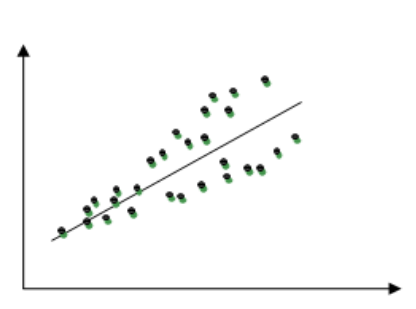
\includegraphics[width=0.5\textwidth]{Heteroskedasticity.png}
        \begin{choices}
            \item Homoskedasticity\\
            同方差性
            \item Non - perfect multicollinearity\\
            非完全多重共线性
            \item Perfect multicollinearity\\
            完全多重共线性
            \item Heteroskedasticity\\
            异方差性
        \end{choices}
        
        \begin{correctanswer}
            D
        \end{correctanswer}
        
        \begin{explanation}
        \textbf{A选项错误。}
        \begin{itemize}
            \item 同方差性（Homoskedasticity）是指在回归模型中，误差项的方差不随自变量的变化而变化，即对于所有的自变量取值，误差项的离散程度是相同的。由散点图可知，误差项的方差可能并非恒定，不符合同方差性的特征。
        \end{itemize}
        \textbf{B选项错误。}
        \begin{itemize}
            \item 非完全多重共线性（Non - perfect multicollinearity）是指自变量之间存在一定的线性关系，但不是完全的线性关系。本题中仅涉及一个自变量（债券投资组合经理的经验年限），不存在多个自变量之间的线性关系问题，所以与非完全多重共线性无关。
        \end{itemize}
        \textbf{C选项错误。}
        \begin{itemize}
            \item 完全多重共线性（Perfect multicollinearity）意味着自变量之间存在精确的线性关系。同样，本题只有一个自变量，不存在自变量之间的线性关系，因此也不符合完全多重共线性的情况。
        \end{itemize}
        \textbf{D选项正确。}
        \begin{itemize}
            \item 异方差性（Heteroskedasticity）是指误差项的方差随自变量的变化而变化。从散点图中可以看出，很误差项的离散程度随着自变量（债券投资组合经理的经验年限）的不同而不同，即存在异方差性。
        \end{itemize}
        \end{explanation}
        
        \checklist{回归分析中异方差性、同方差性和多重共线性的判断（根据散点图特征判断是否存在异方差）}


\begin{question}
    A risk analyst at a hedge fund, Alpha Robin, FRM, is examining a single - factor regression. He makes the following statements. Which statement is incorrect?
    \\一位对冲基金的风险分析师，Alpha Robin，FRM，正在检查单因素回归。他做出了以下陈述。哪一项陈述是不正确的？
    \end{question}
    
    \begin{choices}
        \item Heteroskedasticity exists if the regression residuals are correlated with their lagged values.\\
        如果回归残差与它们的滞后值相关，则存在异方差性。
        \item Heteroskedasticity does not affect the consistency or unbiasedness of the OLS parameter estimator.\\
        异方差不会影响普通最小二乘法（OLS）参数估计量的一致性和无偏性。
        \item When residuals are heteroskedastic, the standard errors are usually unreliable estimates.\\
        当残差存在异方差时，标准误差通常是不可靠的估计。
        \item A consequence of heteroskedasticity is that the asymptotic distribution of the estimated parameters takes a different form.\\
        异方差的一个后果是估计参数的渐近分布会呈现不同的形式。

    \end{choices}
    
    \begin{correctanswer}
    A
    \end{correctanswer}
    
    \begin{explanation}
    \textbf{A选项错误。}
    \begin{itemize}
    \item 回归残差与它们的滞后值相关是自相关的特征，并非异方差的判定依据，所以该选项错误。
    \end{itemize}
    \textbf{B选项正确。}
    \begin{itemize}
    \item 异方差不会影响普通最小二乘法（OLS）参数估计量的一致性和无偏性，该选项表述正确。
    \end{itemize}
    \textbf{C选项正确。}
    \begin{itemize}
        \item 当残差存在异方差时，标准误差通常是不可靠的估计，这会导致假设检验的结果不准确。
    \end{itemize}
    \textbf{D选项正确。}
    \begin{itemize}
        \item 异方差的一个后果是估计参数的渐近分布会呈现不同的形式，通常会影响参数的标准误差和置信区间。
    \end{itemize}
    \end{explanation}
    
    \checklist{异方差的定义及其影响（关键在于准确区分异方差和自相关的概念，以及理解异方差对统计推断的影响）}

\begin{question}
    A financial analyst at an asset management firm is conducting a linear regression analysis of a portfolio's returns against several macro - economic variables. The analysis yields a high coefficient of determination (\(R^{2}\)), but only a few significant t - ratios. Which assumption is most likely violated?
    \\一位资产管理公司的财务分析师正在对投资组合收益率与几个宏观经济变量进行线性回归分析。分析结果显示高决定系数（\(R^{2}\)），但只有少数显著的t比率。哪一项假设最有可能被违反？
    \end{question}
    
    \begin{choices}
        \item Error term is normal with mean = 0 and constant variance = \(\sigma\)\\
        误差项服从均值为0、方数为\(\sigma\)的正态分布
        \item No auto - correlation between error terms\\
        误差项之间不存在自相关
        \item Multicollinearity\\
        多重共线性
        \item Homoscedasticity\\
        同方差性
    \end{choices}
    
    \begin{correctanswer}
        C
    \end{correctanswer}
    
    \begin{explanation}
    \textbf{A选项错误。}
    \begin{itemize}
        \item 误差项服从均值为0、方差为\(\sigma\)的正态分布这一假设被违反时，主要影响的是参数估计的有效性和统计推断的准确性，但通常不会直接导致高 \(R^{2}\) 和低显著t比率的情况。
    \end{itemize}
    \textbf{B选项错误。}
    \begin{itemize}
        \item 误差项不存在自相关的假设被违反时，会影响标准误的计算和统计检验的可靠性，但不是造成高 \(R^{2}\) 和低显著t比率的典型原因。
    \end{itemize}
    \textbf{C选项正确。}
    \begin{itemize}
        \item 多重共线性是指自变量之间存在高度的线性关系。当存在多重共线性时，回归模型可以很好地拟合数据，导致 \(R^{2}\) 较高。然而，由于自变量之间的相关性，很难准确地分离出每个自变量对因变量的单独影响，使得t比率不显著。
    \end{itemize}
    \textbf{D选项错误。}
    \begin{itemize}
        \item 同方差性假设被违反，即存在异方差时，主要影响的是参数估计的效率和标准误的计算，不会直接表现为高 \(R^{2}\) 和低显著t比率。
    \end{itemize}
    \end{explanation}
    
    \checklist{多重共线性（多重共线性在\(R^{2}\)和t值上的表现）}


    \begin{question}
    A junior analyst at a financial consulting firm is analyzing a regression model that estimates the quarterly revenue of a company based on multiple economic indicators. The analyst discovers that the variance of the error term is an increasing function of the explanatory variable. Which assumption of the regression model is violated?
    \\一位金融咨询公司的初级分析师正在分析一个回归模型，该模型根据多个经济指标估计公司的季度收入。分析师发现误差项的方差是解释变量的增函数。哪一项回归模型的假设被违反？
    \end{question}
    
    \begin{choices}
        \item No autocorrelation between error terms\\
        误差项之间不存在自相关
        \item Model is linear\\
        模型是线性的
        \item Multicollinearity\\
        多重共线性
        \item Homoscedasticity\\
        同方差性
    \end{choices}
    
    \begin{correctanswer}
        D
    \end{correctanswer}
    
    \begin{explanation}
    \textbf{A选项错误。}
    \begin{itemize}
        \item 误差项无自相关假设关注的是不同观测值的误差项之间是否存在相关性，而题干描述的是误差项方差与解释变量的关系，并非误差项之间的相关性，所以该假设未被违反。
    \end{itemize}
    \textbf{B选项错误。}
    \begin{itemize}
        \item 模型线性假设强调因变量和自变量之间是线性关系，与误差项方差随解释变量变化这一情况没有直接关联，所以该假设未被违反。
    \end{itemize}
    \textbf{C选项错误。}
    \begin{itemize}
        \item 多重共线性是指自变量之间存在高度的线性关系，它主要影响回归系数的估计和显著性检验，和误差项方差与解释变量的变化关系无关，所以该假设未被违反。
    \end{itemize}
    \textbf{D选项正确。}
    \begin{itemize}
        \item 同方差性假设要求误差项的方差是一个常数，不随解释变量的变化而改变。当误差项的方差是解释变量的增函数时，说明误差项的方差不是恒定的，这就违反了同方差性假设。
    \end{itemize}
    \end{explanation}
    
    \checklist{线性回归模型假设的判断（误差项方差与解释变量相关时违反同方差性假设，会导致异方差问题）}

    \begin{question}
    A risk analyst at an asset management firm is conducting a White test to check for heteroskedasticity in a portfolio. The portfolio is modeled as \(Y_i = \alpha+\beta X_{1i}+\epsilon_i\). The residuals are calculated as \(\hat{\epsilon}_i=Y_i - \hat{\alpha}-\hat{\beta}X_{1i}\). Which of the following equations correctly represents the second step in the White test for this portfolio?
    \\一位资产管理公司的风险分析师正在对投资组合进行怀特检验，以检查投资组合中是否存在异方差。投资组合被建模为 \(Y_i = \alpha+\beta X_{1i}+\epsilon_i\)。残差计算为 \(\hat{\epsilon}_i=Y_i - \hat{\alpha}-\hat{\beta}X_{1i}\)。以下哪个方程正确表示了投资组合的怀特检验的第二步？
    \end{question}
    
    \begin{choices}
        \item \(\hat{\epsilon}_i^2=\gamma_0+\gamma_1X_{1i}+\gamma_2X_{1i}^2+\nu_i\)
        \item \(\hat{\epsilon}_i^2=\gamma_1X_{1i}+\gamma_2X_{1i}^2+\nu_i\)
        \item \(\hat{\epsilon}_i^2=\gamma_0+\gamma_1X_{1i}+\nu_i\)
        \item \(\hat{\epsilon}_i^2=\gamma_0+\gamma_1X_{1i}^2+\nu_i\)
    \end{choices}
    
    \begin{correctanswer}
        A
    \end{correctanswer}
    
    \begin{explanation}
    \textbf{怀特检验（White test）}
    \begin{itemize}
        \item 怀特检验（White test）用于检验回归模型中是否存在异方差性。
        \item 在进行怀特检验时，第二步是将残差的平方\(\hat{\epsilon}_i^2\)对原回归模型中的自变量、自变量的平方以及自变量之间的交叉项进行回归。
        \item 对于模型 \(Y_i = \alpha+\beta X_{1i}+\epsilon_i\)，其怀特检验的第二步回归方程为 \(\hat{\epsilon}_i^2=\gamma_0+\gamma_1X_{1i}+\gamma_2X_{1i}^2+\nu_i\)，这里包含了常数项、自变量 \(X_{1i}\) 以及自变量的平方 \(X_{1i}^2\)，故选项A正确。
    \end{itemize}
    \end{explanation}
    
    \checklist{怀特检验（关键在于理解怀特检验回归方程的构成）}

    \begin{question}
        A junior risk analyst at a large financial institution is tasked with testing for heteroskedasticity in a multiple - regression model. The analyst decides to use the White test. Which of the following statements correctly outlines the procedures of the White test?
        \end{question}
        
        \begin{choices}
            \item The White test first estimates the model and computes the residuals. It then regresses the residuals on a constant and all explanatory variables.
            \item The White test first estimates the model and computes the residuals. It then regresses the squared residuals on a constant and all explanatory variables.
            \item The White test first estimates the model and computes the residuals. It then regresses the squared residuals on a constant, all explanatory variables, their squares, and their cross - product.
            \item The White test first estimates the model and computes the residuals. It then regresses the residuals on a constant, all explanatory variables, their squares, and their cross - product.
        \end{choices}
        
        \begin{correctanswer}
            C
        \end{correctanswer}
        
        \begin{explanation}
        \textbf{怀特检验（White test）}
        \begin{itemize}
            \item 假设原模型有两个解释变量（\(k=2\))：
            \[
            Y_i = \alpha + \beta_1 X_{1i} + \beta_2 X_{2i} + \epsilon_i
            \]
		
            \item 第一步是使用OLS模型计算残差：
            \[
            \hat{\epsilon}_i = Y_i - \hat{\alpha} - \hat{\beta}_1 X_{1i} - \hat{\beta}_2 X_{2i}
            \]
		
            \item 将残差的平方（the squared residuals）对常数、所有解释变量、解释变量的平方以及解释变量之间的交叉乘积项（\(X_1, X_2, X_1^2, X_2^2, X_1X_2\)）进行回归，通过这种方式来检验异方差性:
            \[
            \hat{\epsilon}_i^2 = \gamma_0 + \gamma_1 X_{1i} + \gamma_2 X_{2i} + \gamma_3 X_{1i}^2 + \gamma_4 X_{2i}^2 + \gamma_5 X_{1i}X_{2i} + \eta_i
            \]
            \item 选项C正确。
        \end{itemize}
        \end{explanation}
        
        \checklist{怀特检验的步骤（关键在于准确把握怀特检验中对残差平方进行回归时所包含的变量）}

\begin{question}
A risk analyst at a fixed-income hedge fund is evaluating a yield curve prediction model. To improve the model's accuracy, she is considering adding several macroeconomic indicators such as GDP growth rate, inflation rate, and unemployment rate. When incorporating these potentially irrelevant variables into the regression model, which of the following statements about their impact is incorrect?
\\一位固定收益对冲基金的风险分析师正在评估一个收益率曲线预测模型。为了提高模型的准确性，她考虑添加几个宏观经济指标，如GDP增长率、通胀率和失业率。当将这些潜在无关变量纳入回归模型时，以下哪一项陈述关于它们的影响是不正确的？
\end{question}


\begin{choices}
    \item In a multiple regression model, adding an irrelevant variable will always increase R² as long as its regression coefficient is non-zero.\\
    在多元回归模型中，添加一个无关变量将始终增加R²，只要其回归系数不为零。
    \item After adding an irrelevant explanatory variable, the adjusted R² may either increase or decrease.\\
    添加一个无关解释变量后，调整后的R²可能上升也可能下降。
    \item If the newly added variable has high correlation with existing variables in the model, the standard errors of the regression coefficients will increase.\\
    如果新添加的变量与模型中的现有变量高度相关，回归系数的标准误差将增加。
    \item The addition of irrelevant variables will not affect the mean of residuals.\\
    添加无关变量不会影响残差的均值。
\end{choices}

\begin{correctanswer}
D
\end{correctanswer}

\begin{explanation}
令 \(X_1, X_2, ..., X_k\) 为原模型中的解释变量，\(Z\) 为新加入的无关变量。

\textbf{A选项正确。}
\begin{itemize}
    \item 当加入新变量 \(Z\) 时，R²的计算公式为：
    \[R^2 = 1 - \frac{SSR}{SST} = 1 - \frac{\sum(y_i - \hat{y_i})^2}{\sum(y_i - \bar{y})^2}\]
    \item 只要 \(Z\) 的回归系数 \(\beta_z \neq 0\)，SSR必然减小，导致R²上升。
\end{itemize}

\textbf{B选项正确。}
\begin{itemize}
    \item 调整后的R²计算公式：
    \[\bar{R}^2 = 1 - \frac{n-1}{n-k-1}(1-R^2)\]
    其中 \(n\) 为样本量，\(k\) 为变量个数
    \item 加入 \(Z\) 后，\(k\) 增加，分母 \(n-k-1\) 减小，同时R²增加
    \item 这两个相反的效应导致 \(\bar{R}^2\) 可能上升也可能下降
\end{itemize}

\textbf{C选项正确。}
\begin{itemize}
    \item 当新变量 \(Z\) 与现有变量高度相关时，存在：
    \[Corr(X_i, Z) \approx \pm 1\]
    \item 这会导致方差膨胀因子（VIF）增大：
    \[VIF = \frac{1}{1-R^2_i}\]
    其中 \(R^2_i\) 是第 \(i\) 个变量对其他变量的回归R²
    \item 因此回归系数的标准误差增大：
    \[SE(\hat{\beta_i}) = \sqrt{\frac{\sigma^2}{SST_i(1-R^2_i)}}\]
\end{itemize}

\textbf{D选项错误。}
\begin{itemize}
    \item 加入无关变量会影响残差项的均值。设原模型为：
    \[y = X\beta + \varepsilon\]
    \item 加入 \(Z\) 后模型变为：
    \[y = X\beta + Z\gamma + \varepsilon'\]
    \item 新的残差 \(\varepsilon'\) 与原残差 \(\varepsilon\) 不同，其均值可能发生变化，这相当于将原本存在于残差项中的某些变异"分离"出来，必然影响残差的分布特征。
\end{itemize}
\end{explanation}

\checklist{回归模型中无关变量的影响（关键是理解对R²、调整R²、标准误和残差的影响）}
\begin{question}
An analyst conducts three separate regressions (all coefficients estimated using OLS method) on three variables: stock S returns, gold commodity returns, and US 1-year Treasury bill returns. The regression results are shown in the table below. Based on the information in the table, which of the following statements is correct?

\begin{center}
\begin{table}[H]
\centering
\caption{Results of Three Regressions}
\begin{tabular}{lccc}
\toprule
Model & Regression Equation & \(\beta_0\) & \(\beta_1\) \\
\midrule
\multirow{4}{*}{Regression 1} & Stock = \(\beta_0 + \beta_1\) × Gold & -0.0003 & 0.57 \\
& Standard Error & 0.0002 & 0.028 \\
& t-statistic & -1.5 & 20.36 \\
& \(R^2\) & \multicolumn{2}{c}{0.45} \\
\midrule
\multirow{4}{*}{Regression 2} & Stock = \(\beta_0 + \beta_1\) × Bill & -0.0003 & 2.28 \\
& Standard Error & 0.0004 & 0.053 \\
& t-statistic & -0.75 & 43.02 \\
& \(R^2\) & \multicolumn{2}{c}{0.70} \\
\midrule
\multirow{4}{*}{Regression 3} & Gold = \(\beta_0 + \beta_1\) × Bill & 0.0002 & 0.054 \\
& Standard Error & 0.0004 & 0.015 \\
& t-statistic & 0.50 & 3.60 \\
& \(R^2\) & \multicolumn{2}{c}{0.37} \\
\bottomrule
\end{tabular}
\end{table}
\end{center}
一位分析师对三个变量进行了三次独立的回归（所有系数均使用OLS方法估计）：股票S收益率、黄金商品收益率和美国1年期国债收益率。回归结果如下表所示。根据表中的信息，下列关于这些陈述的陈述中，哪一项是正确的？

\begin{center}
\begin{table}[H]
\centering
\caption{三次回归的结果}
\begin{tabular}{lccc}
\toprule
模型 & 回归方程 & \(\beta_0\) & \(\beta_1\) \\
\midrule
\multirow{4}{*}{回归1} & 股票 = \(\beta_0 + \beta_1\) × 黄金 & -0.0003 & 0.57 \\
& 标准误 & 0.0002 & 0.028 \\
& t统计量 & -1.5 & 20.36 \\
& \(R^2\) & \multicolumn{2}{c}{0.45} \\
\midrule
\multirow{4}{*}{回归2} & 股票 = \(\beta_0 + \beta_1\) × 国债 & -0.0003 & 2.28 \\
& 标准误 & 0.0004 & 0.053 \\
& t统计量 & -0.75 & 43.02 \\
& \(R^2\) & \multicolumn{2}{c}{0.70} \\
\midrule
\multirow{4}{*}{回归3} & 黄金 = \(\beta_0 + \beta_1\) × 国债 & 0.0002 & 0.054 \\
& 标准误 & 0.0004 & 0.015 \\
& t统计量 & 0.50 & 3.60 \\
& \(R^2\) & \multicolumn{2}{c}{0.37} \\
\bottomrule
\end{tabular}
\end{table}
\end{center}
\end{question}

\begin{choices}
    \item Due to omitted variable bias, the coefficient of gold returns in Regression 1 is overestimated\\
    由于遗漏变量偏误，回归1中黄金收益率的系数被高估
    \item Due to heteroskedasticity, the coefficient of Treasury bill returns in Regression 2 is overestimated\\
    由于异方差，回归2中国债收益率的系数被高估
    \item The intercept term in Regression 3 is significantly different from zero\\
    回归3中的截距项在统计上显著异于0
    \item Due to multicollinearity, the \(R^2\) in Regression 2 is high\\
    由于多重共线性，回归2中的R²很高
\end{choices}

\begin{correctanswer}
A
\end{correctanswer}

\begin{explanation}
\textbf{A选项正确。}
\begin{itemize}
    \item 遗漏变量偏误需要满足两个条件：
    \begin{enumerate}
        \item 遗漏变量与已包含的自变量相关
        \item 遗漏变量对因变量有显著影响
    \end{enumerate}
    
    \item 从回归3可以看出，Bill与Gold显著相关（t = 3.6），从回归2可以看出，Bill对Stock有显著影响（t = 43.02），因此在回归1中遗漏了Bill这个变量，导致Gold的系数被高估。
\end{itemize}

\begin{figure}[H]
\centering
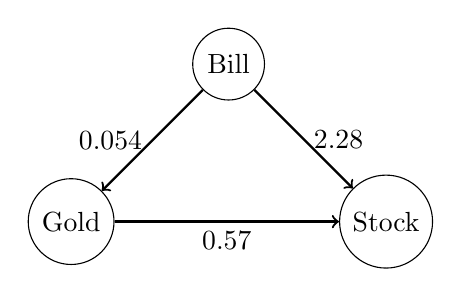
\begin{tikzpicture}
\node[draw, circle] (Gold) at (0,0) {Gold};
\node[draw, circle] (Stock) at (4,0) {Stock};
\node[draw, circle] (Bill) at (2,2) {Bill};
\draw[->, thick] (Gold) -- (Stock) node[midway, below] {0.57};
\draw[->, thick] (Bill) -- (Stock) node[midway, right] {2.28};
\draw[->, thick] (Bill) -- (Gold) node[midway, left] {0.054};
\end{tikzpicture}
\caption{变量间的关系图}
\end{figure}


\textbf{B选项错误。}
\begin{itemize}
    \item 异方差性的判断需要以下证据之一：
    \begin{enumerate}
        \item 残差图显示残差随自变量变化而变化
        \item 通过White检验或BP检验等统计检验
        \item 标准误随自变量变化而系统性变化
    \end{enumerate}
    \item 表中只给出了回归2的系数(2.28)和标准误(0.053)，t统计量(43.02)显著，但这些信息都不足以判断是否存在异方差问题。
\end{itemize}

\textbf{C选项错误。}
\begin{itemize}
    \item 判断截距项是否显著需要比较t统计量与临界值：
    \begin{enumerate}
        \item 回归3中截距项的t统计量为0.50
        \item 在通常的显著性水平下（如5\%），双尾检验的临界值约为±1.96
        \item 0.50 < 1.96，因此不能拒绝"截距项为0"的原假设
    \end{enumerate}
    \item 这表明回归3的截距项在统计上不显著异于0
\end{itemize}

\textbf{D选项错误。}
\begin{itemize}
    \item 多重共线性的判断条件：
    \begin{enumerate}
        \item 需要至少两个解释变量之间存在高度相关性
        \item 通常通过VIF > 10或相关系数接近±1来判断
    \end{enumerate}
    \item 回归2中只有一个解释变量（Bill），不存在与其他解释变量的相关性问题，R²=0.70的高值是由于Bill对Stock具有较强的解释能力（t=43.02），而非多重共线性导致。
\end{itemize}
\end{explanation}

\checklist{遗漏变量偏误的判断（关键是判断遗漏变量与已有变量的相关性，以及对因变量的影响）}

\end{document}